\documentclass[a4paper,12pt, spanish]{report}
\usepackage[utf8]{inputenc}
\usepackage{enumitem} %permite el uso de letras para enumerar
\usepackage{graphicx} %para las imágenes
\usepackage{float} %para fijar las imágenes
\usepackage{booktabs} %para fijar las imágenes
\usepackage{wrapfig} %para que el texto se acomode entre las imagenes
\usepackage[spanish]{babel}
\renewcommand{\arraystretch}{2} % Escala la altura de las filas
\usepackage{multirow}
\usepackage[table]{xcolor}

\usepackage{amsmath}%para entornos de alineación
\usepackage{amsfonts}%para las letras lindas de matemática
\usepackage{xfrac}%para fracciones chiquitas
\allowdisplaybreaks
\setlength{\jot}{8pt}%modifica el interlineado
\usepackage[font=footnotesize,labelfont=bf]{caption}

\usepackage{pgfplots}

\usepackage{tikz} %Librería para gráficos
\usetikzlibrary{calc, arrows.meta, positioning}

\usepackage[a4paper, %margenes de pagina
  left=2.5cm,
  right=2.5cm,
  top=2cm,
  bottom=2cm,
  includehead
]{geometry}

\usepackage{fancyhdr}
\pagestyle{fancy}
\lhead{UTN-FRC}
\chead{Dispisitivos Electronicos I}
\rhead{3R2}
\cfoot{\thepage}
\setlength{\headwidth}{\textwidth} % Hace que el ancho del encabezado coincida con el ancho del texto
\setlength{\headheight}{15pt}  % Ajusta la altura del encabezado
\setlength{\headsep}{20pt}     % Ajusta la separación entre el encabezado y el contenido

\usepackage{titlesec}
\titleformat{\chapter}[display]{\normalfont\Large\bfseries}{}{0pt}{}
\titlespacing*{\chapter}{10pt}{-45pt}{10pt}

\usepackage{etoolbox} 
\makeatletter
\patchcmd{\chapter}{\thispagestyle{plain}}{\thispagestyle{fancy}}{}{} %Muestra encabezado en las paginas con \chapter
\makeatother

%Comandos de fake section y fake sub section, para poder agregar secciones al indice
\newcommand{\fs}[1]{%
  \par\refstepcounter{section}% Increase section counter
  \sectionmark{#1}% Add section mark (header)
  \addcontentsline{toc}{section}{\protect\numberline{\thechapter.\alph{section}}#1}% Add section to ToC
}
\newcommand{\fss}[1]{%
  \par\refstepcounter{subsection}% Increase subsection counter
  \subsectionmark{#1}% Add subsection mark (header)
  \addcontentsline{toc}{subsection}{\protect\numberline{\alph{subsection}}#1}% Add subsection to ToC
}

\usepackage{afterpage}
\newcommand\myemptypage{
  \newpage
  \null
  \thispagestyle{empty}
  \addtocounter{page}{-1}
  \newpage
}

\usepackage{circuitikz}

\title{%
\setlength{\headwidth}{\textwidth} % Hace que el encabezado tenga el mismo ancho que el contenido
\setlength{\headheight}{15pt}  % Ajusta la altura del encabezado
\setlength{\headsep}{10pt}     % Ajusta la separación entre el encabezado y el contenido
  \fontsize{25}{0}\selectfont Universidad Tecnológica Nacional \\
  \fontsize{22}{30}\selectfont Dispositivos Electrónicos I \\
  \fontsize{20}{25}\selectfont Trabajo Practico N° 1
}
\author{
  Santino Noccetti - 405927\\
  Franco Palombo - 401910\\
}
\date{08 / 04 / 2025}

\begin{document}

  \maketitle

  \myemptypage

  \tableofcontents
  \thispagestyle{plain}

  \myemptypage

  \chapter{Introducción}
    En este trabajo de laboratorio se propuso el análisis y medición de un circuito puramente resistivo, constando así de 3
    partes fundamentales.

    El primero es el calculo tanto de la corriente como el voltaje que es atravesada/caída por cada resistor,
    teniendo así que utilizar las leyes de Kirchoff, las leyes de Ohm, y la posterior deducción de un sistema de
    ecuaciones para el calculo de todos los parámetros.

    Luego, utilizando el programa LTSpice, se arma el mismo circuito, se simula y mide nuevamente la corriente y el
    voltaje, teniendo así una forma de verificar los valores ideales que calculamos previamente utilizando las leyes
    de Kirchoff y Ohm.

    Como una actividad anexa, el profesor propuso que utilizando un generador de funciones y un osciloscopio, podamos
    experimentar con corriente alterna, y ver como se comportan dichos componentes resistivos cuando se les aplican ese
    tipo de corrientes. También, la actividad anexa sirve el propósito de aprender a usar herramientas nuevas.

    Por ultimo, en la facultad se realiza el procedimiento de armado del circuito y toma de mediciones del mismo.
    La facultad nos proporciono diferentes elementos, entre ellos, una fuente de alimentación de corriente continua,
    registrada como F-44, un generador de funciones GwInstek SFG-2120, registrado como G-174, y por ultimo, el
    osciloscopio LEADER 8041 de 40MHz, registrado como O-98 en conjunto con una sonda. Para la medición de parámetros
    continuos, alternos y corrientes, el grupo proporciono un voltímetro UNI-T modelo UT33A+.

  \myemptypage
  \chapter{Actividad Practica}
    \section{Cálculos}
    \vspace{-0.6cm}
      \begin{figure}[h]
        \centering
        \begin{minipage}{0.7\textwidth}
          \centering
          \begin{circuitikz}[american voltages]
              % nodos
              \draw
                (0, -1) to [V=$V_s$, on grid, invert]                   (0, 3)
                        to [short, -, i>^=$I_t$, on grid]               (1, 3)
                        to [R=$R_1$, v=$V_{R_1}$, on grid]              (4, 3)
                        to [short, -*, on grid]                         (5, 3)
                        to [short, -, on grid]                          (8, 3)
                        to [short, -, i>^=$I_3$, on grid]               (8, 2)
                        to [R=$R_3$, v=$V_{R_3}$, on grid]              (8, 0)
                        to [short, -, on grid]                          (8, -1)
                        to [short, -*, on grid]                         (5, -1)
                        to [short, -, on grid]                          (0, -1)
                        to [short, -, on grid]                          (0, -1)
                (5, 3)  to [short, -, i>^=$I_2$, on grid]               (5, 2)
                        to [R=$R_2$, v=$V_{R_2}$, on grid]              (5, 0)
                        to [short, -, on grid]                          (5, -1)
                ;
          \end{circuitikz}
        \end{minipage}
        \centering
        \begin{minipage}{0.2\textwidth}
          \centering
          \begin{align*}
            V_s &= 10V\\
            R_1 &= 10K\Omega\\
            R_2 &= 4K7\Omega\\
            R_3 &= 3K3\Omega
          \end{align*}
        \end{minipage}
      \end{figure}

      Ecuaciones del Circuito:
      \begin{gather*}
        \begin{cases}
          M_1: &-V_s + V_{R_1} + V_{R_2} = 0\\
          M_2: &-V_s + V_{R_1} + V_{R_3} = 0\\
          &I_2 + I_3 = I_t
        \end{cases}
      \end{gather*}

      Sabiendo que, por ley de Ohm, la caída de tensión en cualquier resistor es:
      \begin{equation}
        V_R = R I
      \end{equation}
      donde $R$ es la resistencia de dicho resistor, e $I$ la intensidad de corriente que pasa por ese resistor,
      podemos entonces despejar la caída de tensión en la $R_1$ reemplazando la caída de tensión de la $R_2$ en la ec.
      de la malla $M_1$:
      \begin{figure}[!h]
        \centering
        \begin{minipage}{0.6\textwidth}
          \centering
          \begin{align*}
            -V_s + V_{R_1} + V_{R_2} &= 0\\
            -V_s + V_{R_1} + R_2 I_2 &= 0\\
            -V_s + V_{R_1} + R_2 (I_t - I_3) &= 0\tag*{\hfill(\ref{i2_sub})}\\
            -V_s + V_{R_1} + R_2 \left(\frac{V_{R_1}}{R_1} - \frac{V_{R_3}}{R_3}\right) &= 0\tag*{\hfill(\ref{it_sub})(\ref{i3_sub})}\\
            -V_s + V_{R_1} + V_{R_1} \frac{R_2}{R_1} - (V_s - V_{R_1}) \frac{R_2}{R_3} &= 0\tag*{\hfill(\ref{vr3_sub})}\\
            V_{R_1} + V_{R_1} \frac{R_2}{R_1} + V_{R-1} \frac{R_2}{R_3} &= V_s \left(1 + \frac{R_2}{R_3}\right)\\
            V_{R_1} \left(1 + \frac{R_2}{R_1} + \frac{R_2}{R_3}\right) &= V_s \left(1 + \frac{R_2}{R_3}\right)\\
            V_{R_1} &= \frac{V_s \left(1 + \frac{R_2}{R_3}\right)}{1 + \frac{R_2}{R_1} + \frac{R_2}{R_3}}
          \end{align*}
        \end{minipage}
        \vline
        \centering
        \begin{minipage}{0.35\textwidth}
          \centering
          \textit{Cálculos Auxiliares}
          \begin{align}
            I_2 + I_3 &= I_t\nonumber\\
            I_2 &= I_t - I_3\tag{a}
            \label{i2_sub}
          \end{align}
          \begin{align}
            V_{R_1} &= R_1 I_t\nonumber\\
            \frac{V_{R_1}}{R_1} &= I_t\tag{b}
            \label{it_sub}
          \end{align}
          \begin{align}
            V_{R_3} &= R_3 I_3\nonumber\\
            \frac{V_{R_3}}{R_3} &= I_3\tag{c}
            \label{i3_sub}
          \end{align}
          \begin{align}
            -V_s + V_{R_1} + V_{R_3} &= 0\nonumber\\
            V_{R_3} &= V_s - V_{R_1}\tag{d}
            \label{vr3_sub}
          \end{align}
        \end{minipage}
      \end{figure}

      Con la ecuación para $V_{R_1}$ podemos despejar $V_{R_2}$, y por consecuente $V_{R_3}$, que son iguales debido a
      que la caída de tensión para resistores en paralelo es la misma. Entonces, reemplazando valores obtenemos:
      \begin{figure}[!h]
        \centering
        \begin{minipage}{0.4\textwidth}
          \begin{align*}
            V_{R_1} &= \frac{V_s \left(1 + \frac{R_2}{R_3}\right)}{1 + \frac{R_2}{R_1} + \frac{R_2}{R_3}}\\
            V_{R_1} &= \frac{10V \left(1 + \frac{4700\Omega}{3300\Omega}\right)}{1 + \frac{4700\Omega}{10000\Omega} + \frac{4700\Omega}{3300\Omega}}\\
            V_{R_1} &= 8,3760V
          \end{align*}
        \end{minipage}
        \centering
        \begin{minipage}{0.4\textwidth}
          \begin{align*}
            V_{R_2} &= V_{R_3}\\
            V_{R_3} &= V_s - V_{R_1}\\
            V_{R_3} &= 10V - 8,3760V\\
            V_{R_3} &= 1,6239V
          \end{align*}
        \end{minipage}
      \end{figure}

      Ahora, con la ley de Ohm, podemos calcular las corrientes que pasan por los resistores:
      \begin{figure}[!h]
      \centering
      \begin{minipage}{0.3\textwidth}
        \begin{align*}
          I_{R_1} &= I_t\\
          I_t &= \frac{V_{R_1}}{R_1}\\
          I_t &= \frac{8,3760V}{10000\Omega}\\
          I_t &= 837,6\mu A
        \end{align*}
      \end{minipage}
      \centering
      \begin{minipage}{0.3\textwidth}
        \begin{align*}
          I_{R_2} &= I_2\\
          I_2 &= \frac{V_{R_2}}{R_2}\\
          I_2 &= \frac{1,6239V}{4700\Omega}\\
          I_2 &= 345,5\mu A
        \end{align*}
      \end{minipage}
      \centering
      \begin{minipage}{0.3\textwidth}
        \begin{align*}
          I_{R_3} &= I_3\\
          I_3 &= \frac{V_{R_3}}{R_3}\\
          I_3 &= \frac{1,6239V}{3300\Omega}\\
          I_3 &= 492\mu A
        \end{align*}
      \end{minipage}
      \end{figure}
      
      \section{Simulación}
      Para la simulación, se utilizo el software LTSpice, en el cual se modelo el circuito, y utilizando el análisis de
      punto de operación (op ó operating point) podemos obtener las corrientes de los resistores y la caída de
      tensión del paralelo de resistores:
      \begin{figure}[!h]
        \centering
        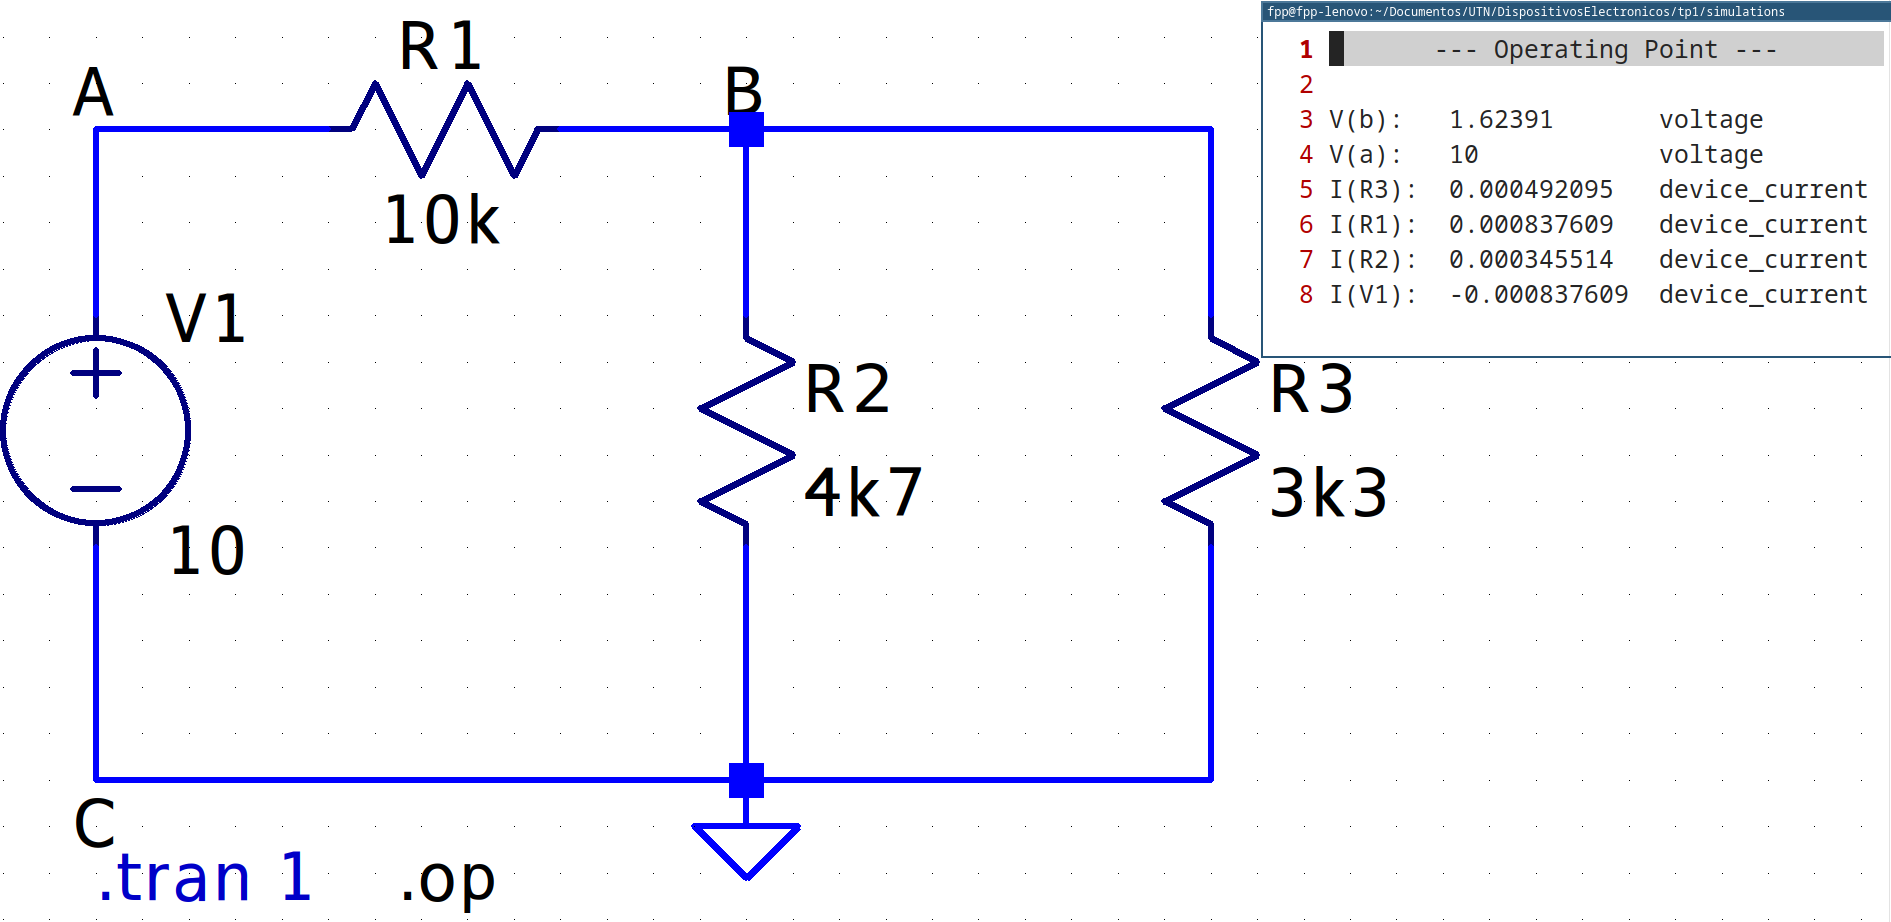
\includegraphics[width=0.8\linewidth]{images/sim_dc.png}

        \caption{Simulación de punto de operación del circuito.}
      \end{figure}

      \section{Implementación y Mediciones}
      \begin{figure}[!h]
        \centering
        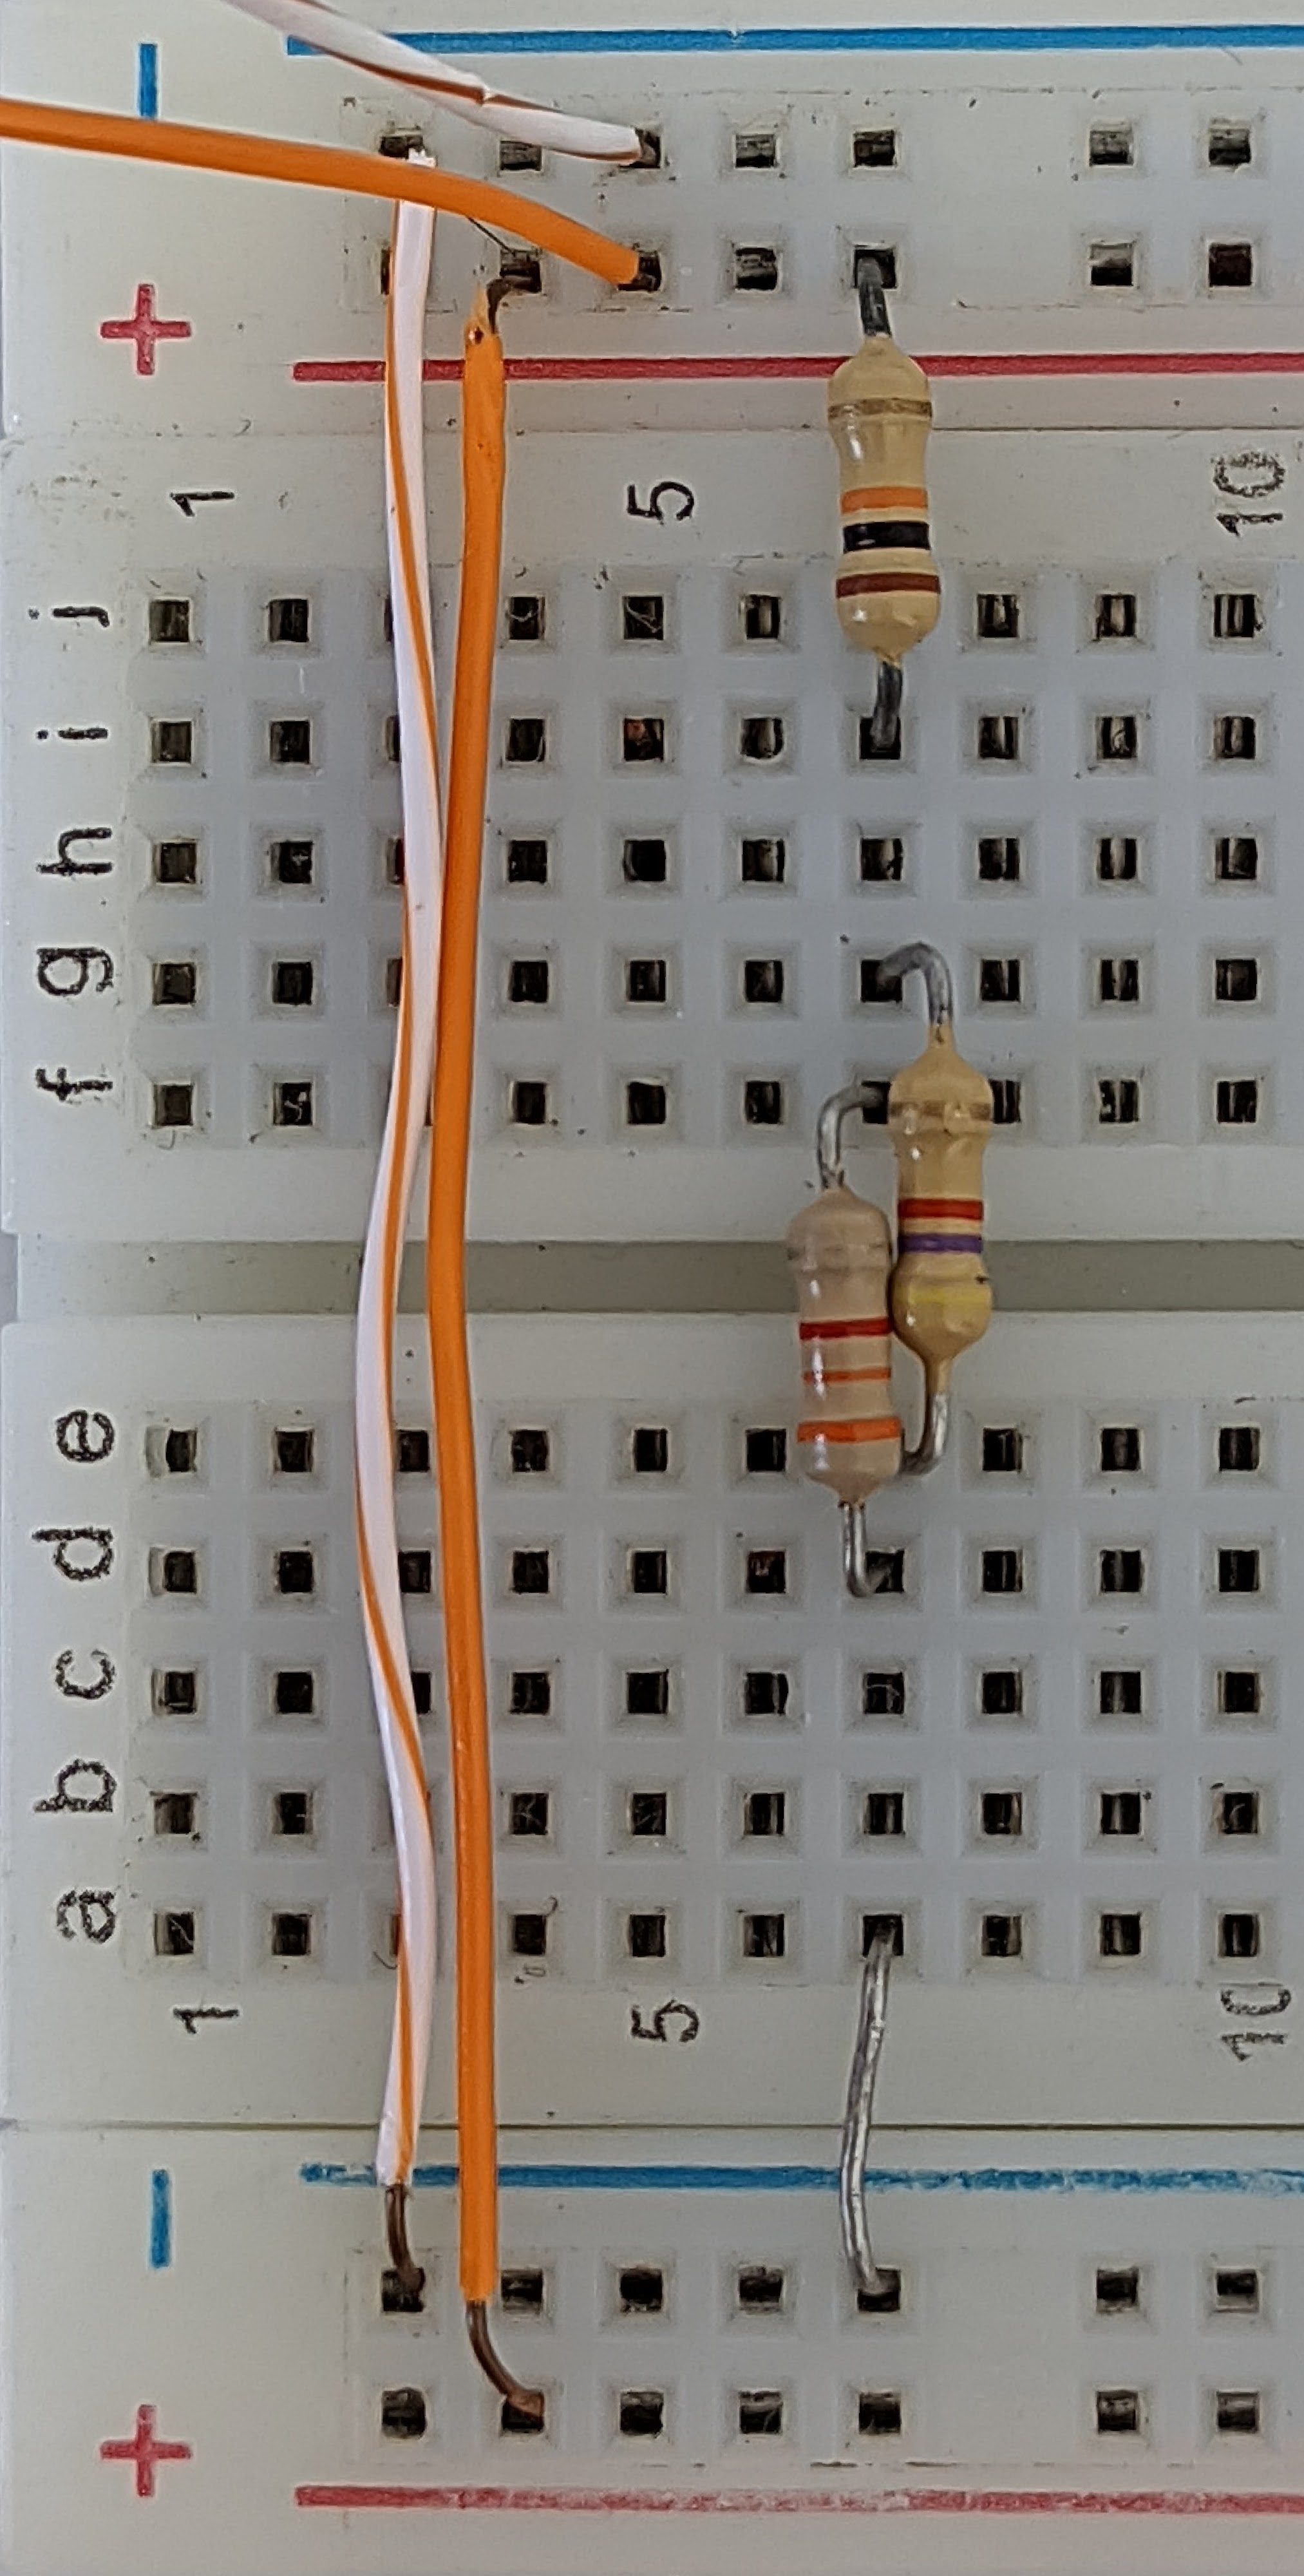
\includegraphics[angle=270, width=0.8\textwidth]{pictures/prot-crkt.jpg}
        \caption{Implementación del circuito.}
        \label{prot-crkt}
      \end{figure}
      \begin{wrapfigure}{r}{0.3\textwidth}
        \vspace{-0.3cm}
        \centering
        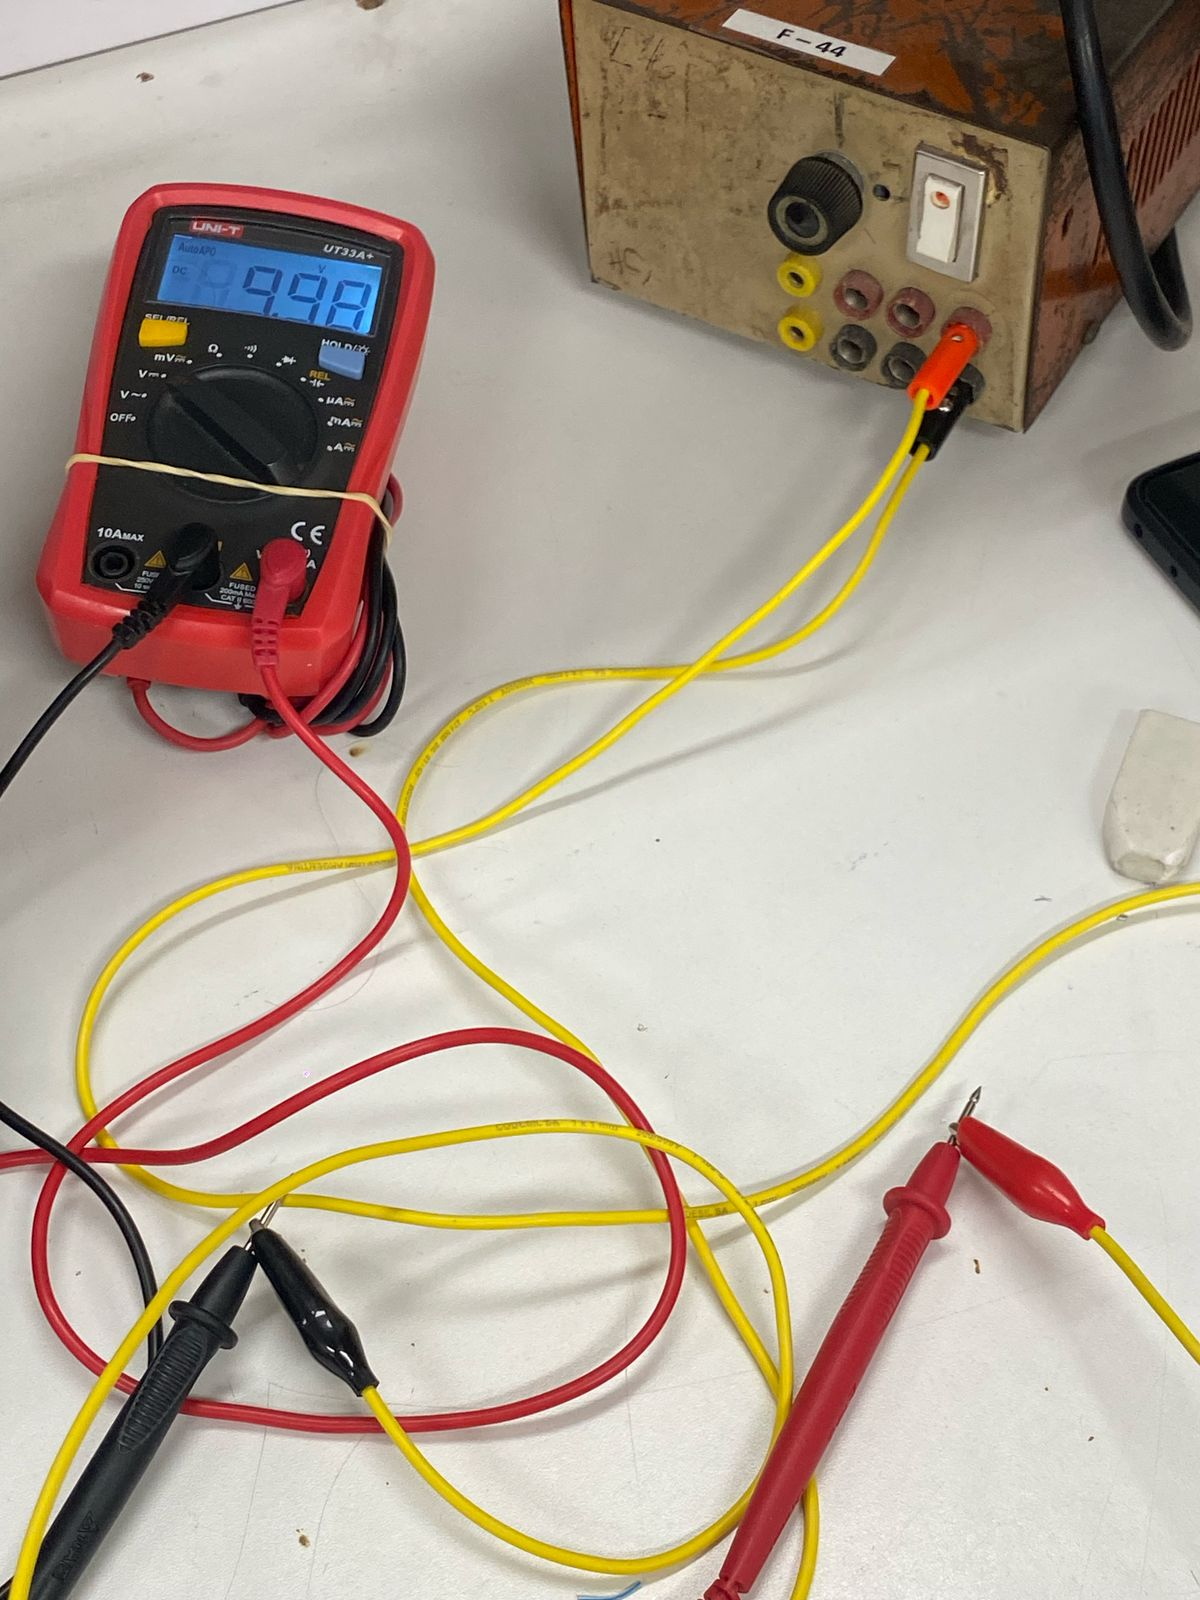
\includegraphics[width=0.25\textwidth]{pictures/mult-vs.jpeg}
        \caption{Calibración de la Fuente.}
        \label{mult-vs}
      \end{wrapfigure}
      Para la implementación del circuito utilizamos una Protoboard, en conjunto con cables unifilares para hacer 
      las conexiones, y resistores de carbono de $\tfrac{1}{4}W$. El circuito quedo como se ve en la figura 
      \ref{prot-crkt}.

      Seguido al ensamblaje del circuito, procedimos a conectar la fuente y calibrar la salida de voltaje lo mas
      próximo a 10V usando el multímetro, como se ve en la figura \ref{mult-vs}. La medición exacta es $9,98V$.

      Después de haber calibrado la fuente, procedimos a conectar los cables banana-cocodrilo al circuito ensamblado
      en la Protoboard y comenzar con las mediciones. A continuación se muestran una serie de imágenes en las que por
      un lado se muestra la medición del multímetro y por otro lado se muestra donde estaban tocando las puntas del
      multímetro.
      \begin{figure}[H]
        \centering
          \begin{minipage}{0.3\textwidth}
            \centering
            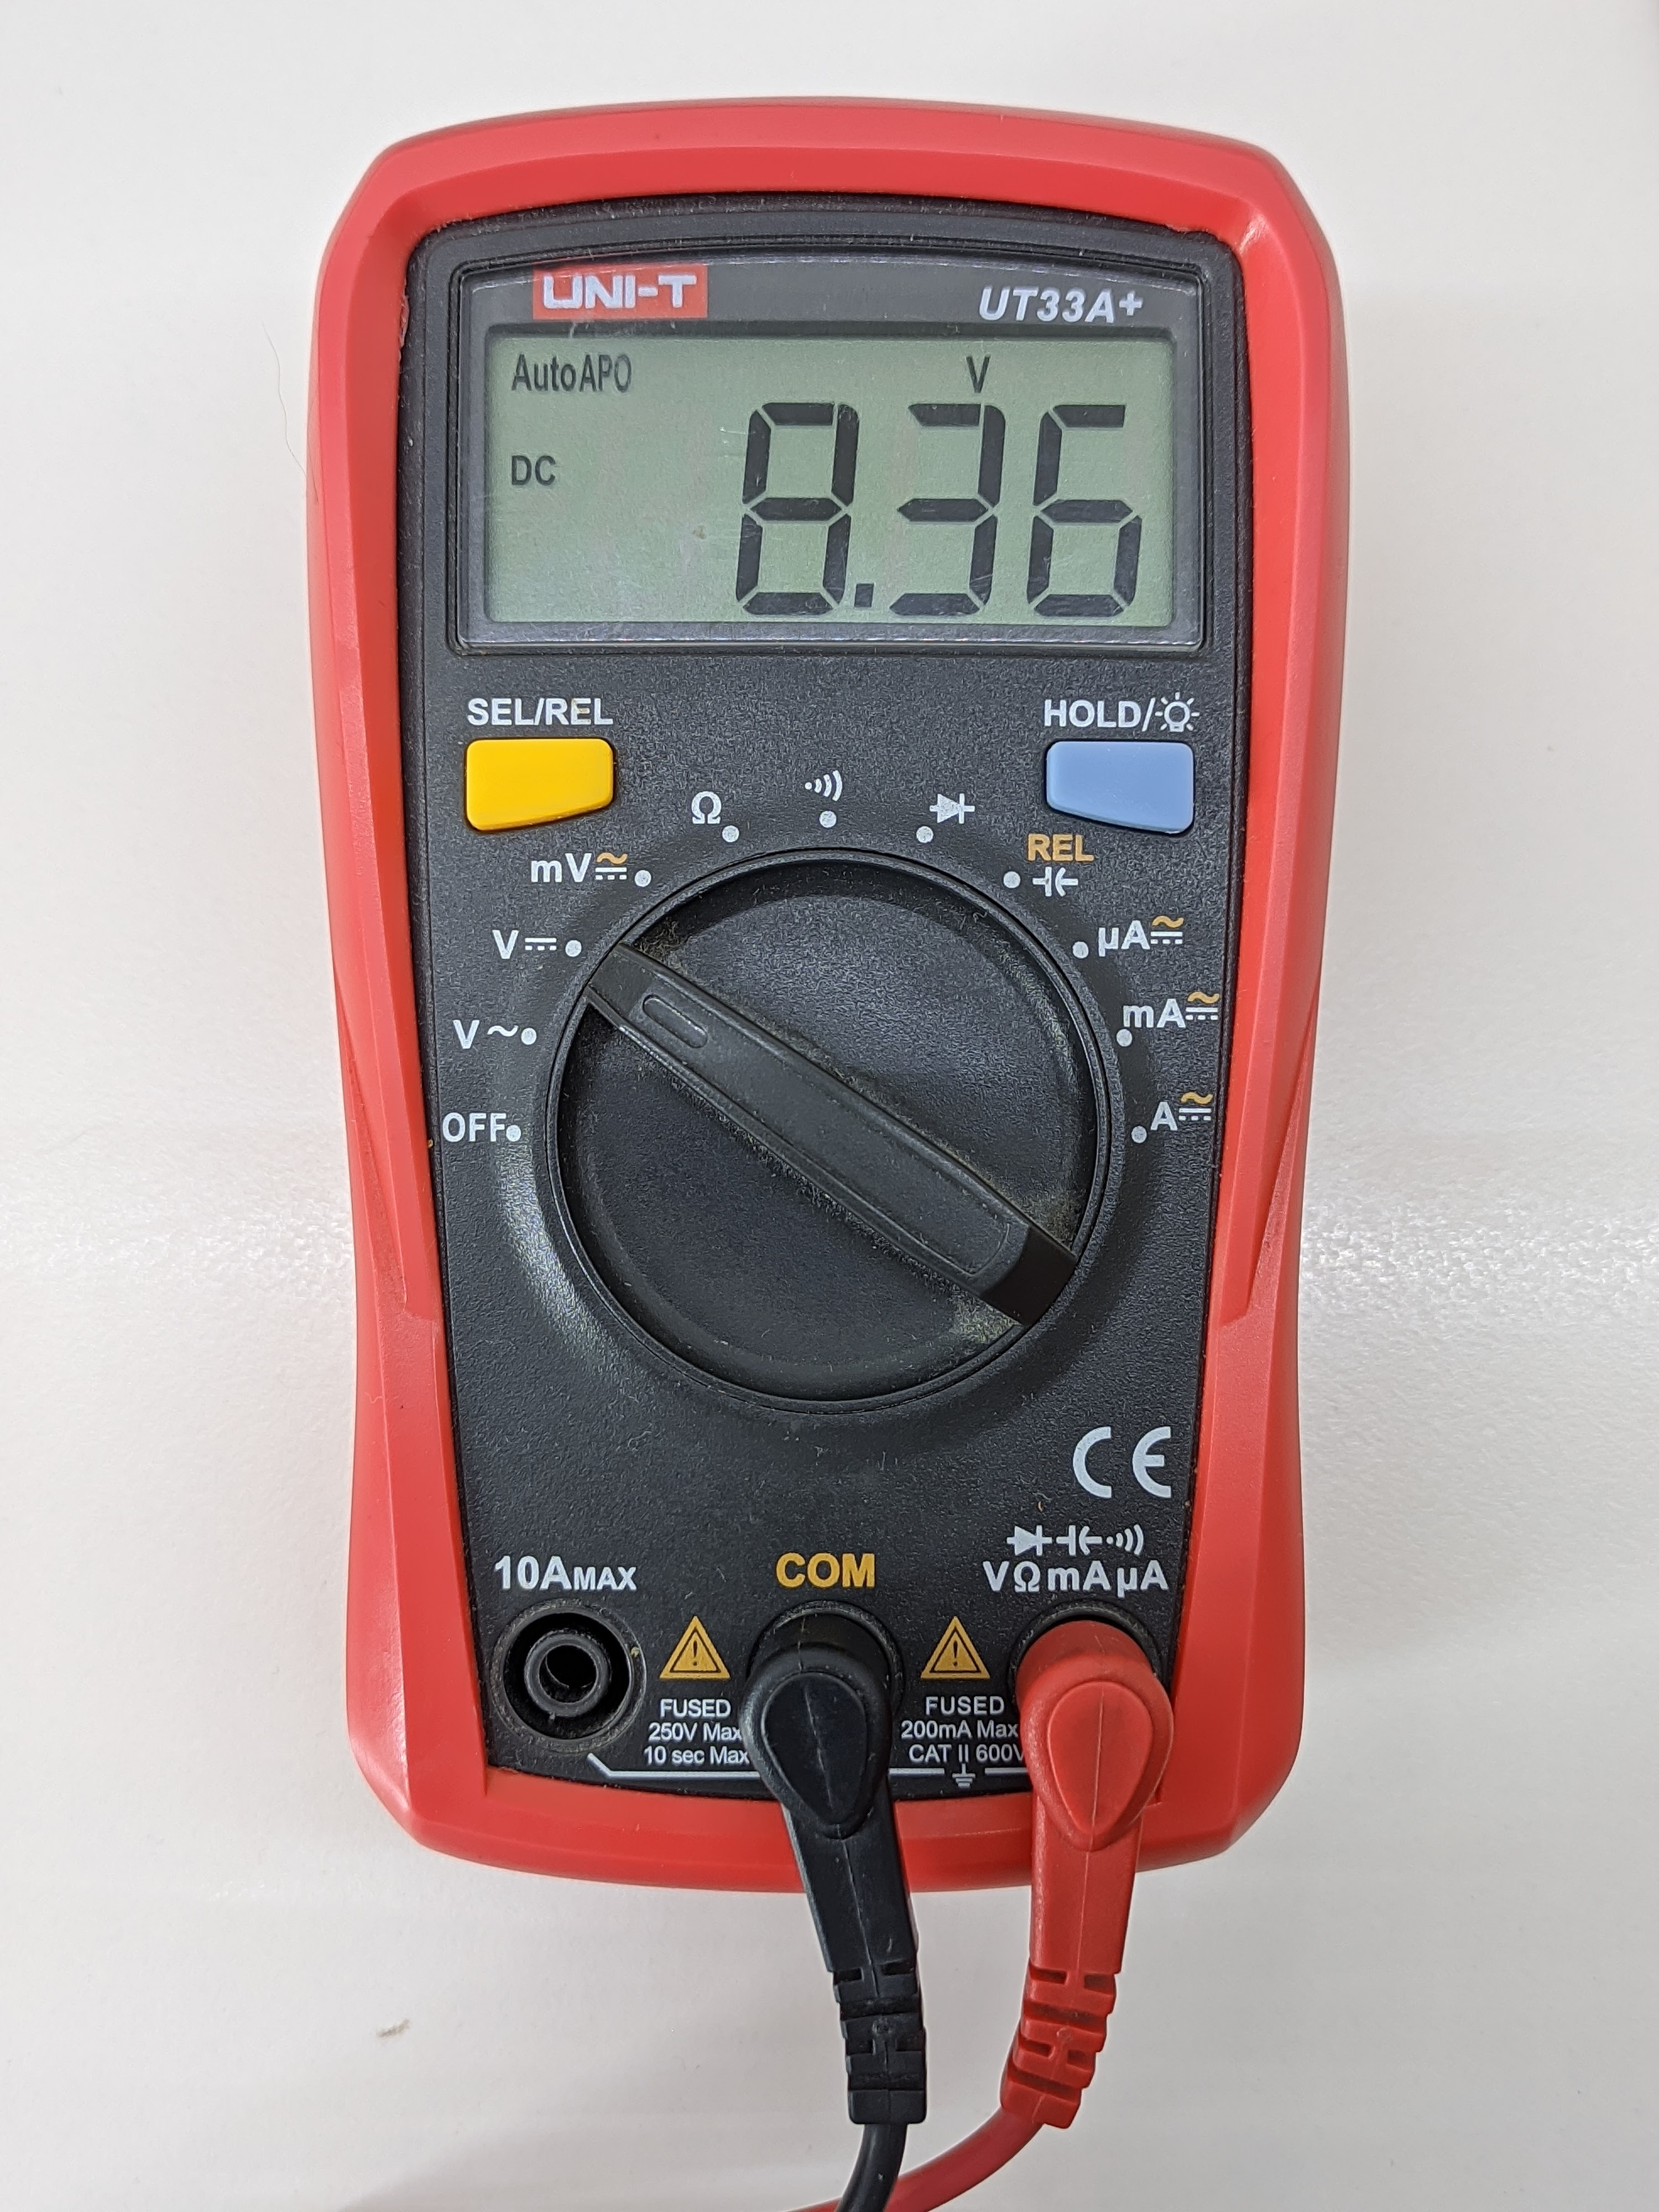
\includegraphics[width=1\linewidth]{pictures/mult-v_r1.jpg}
            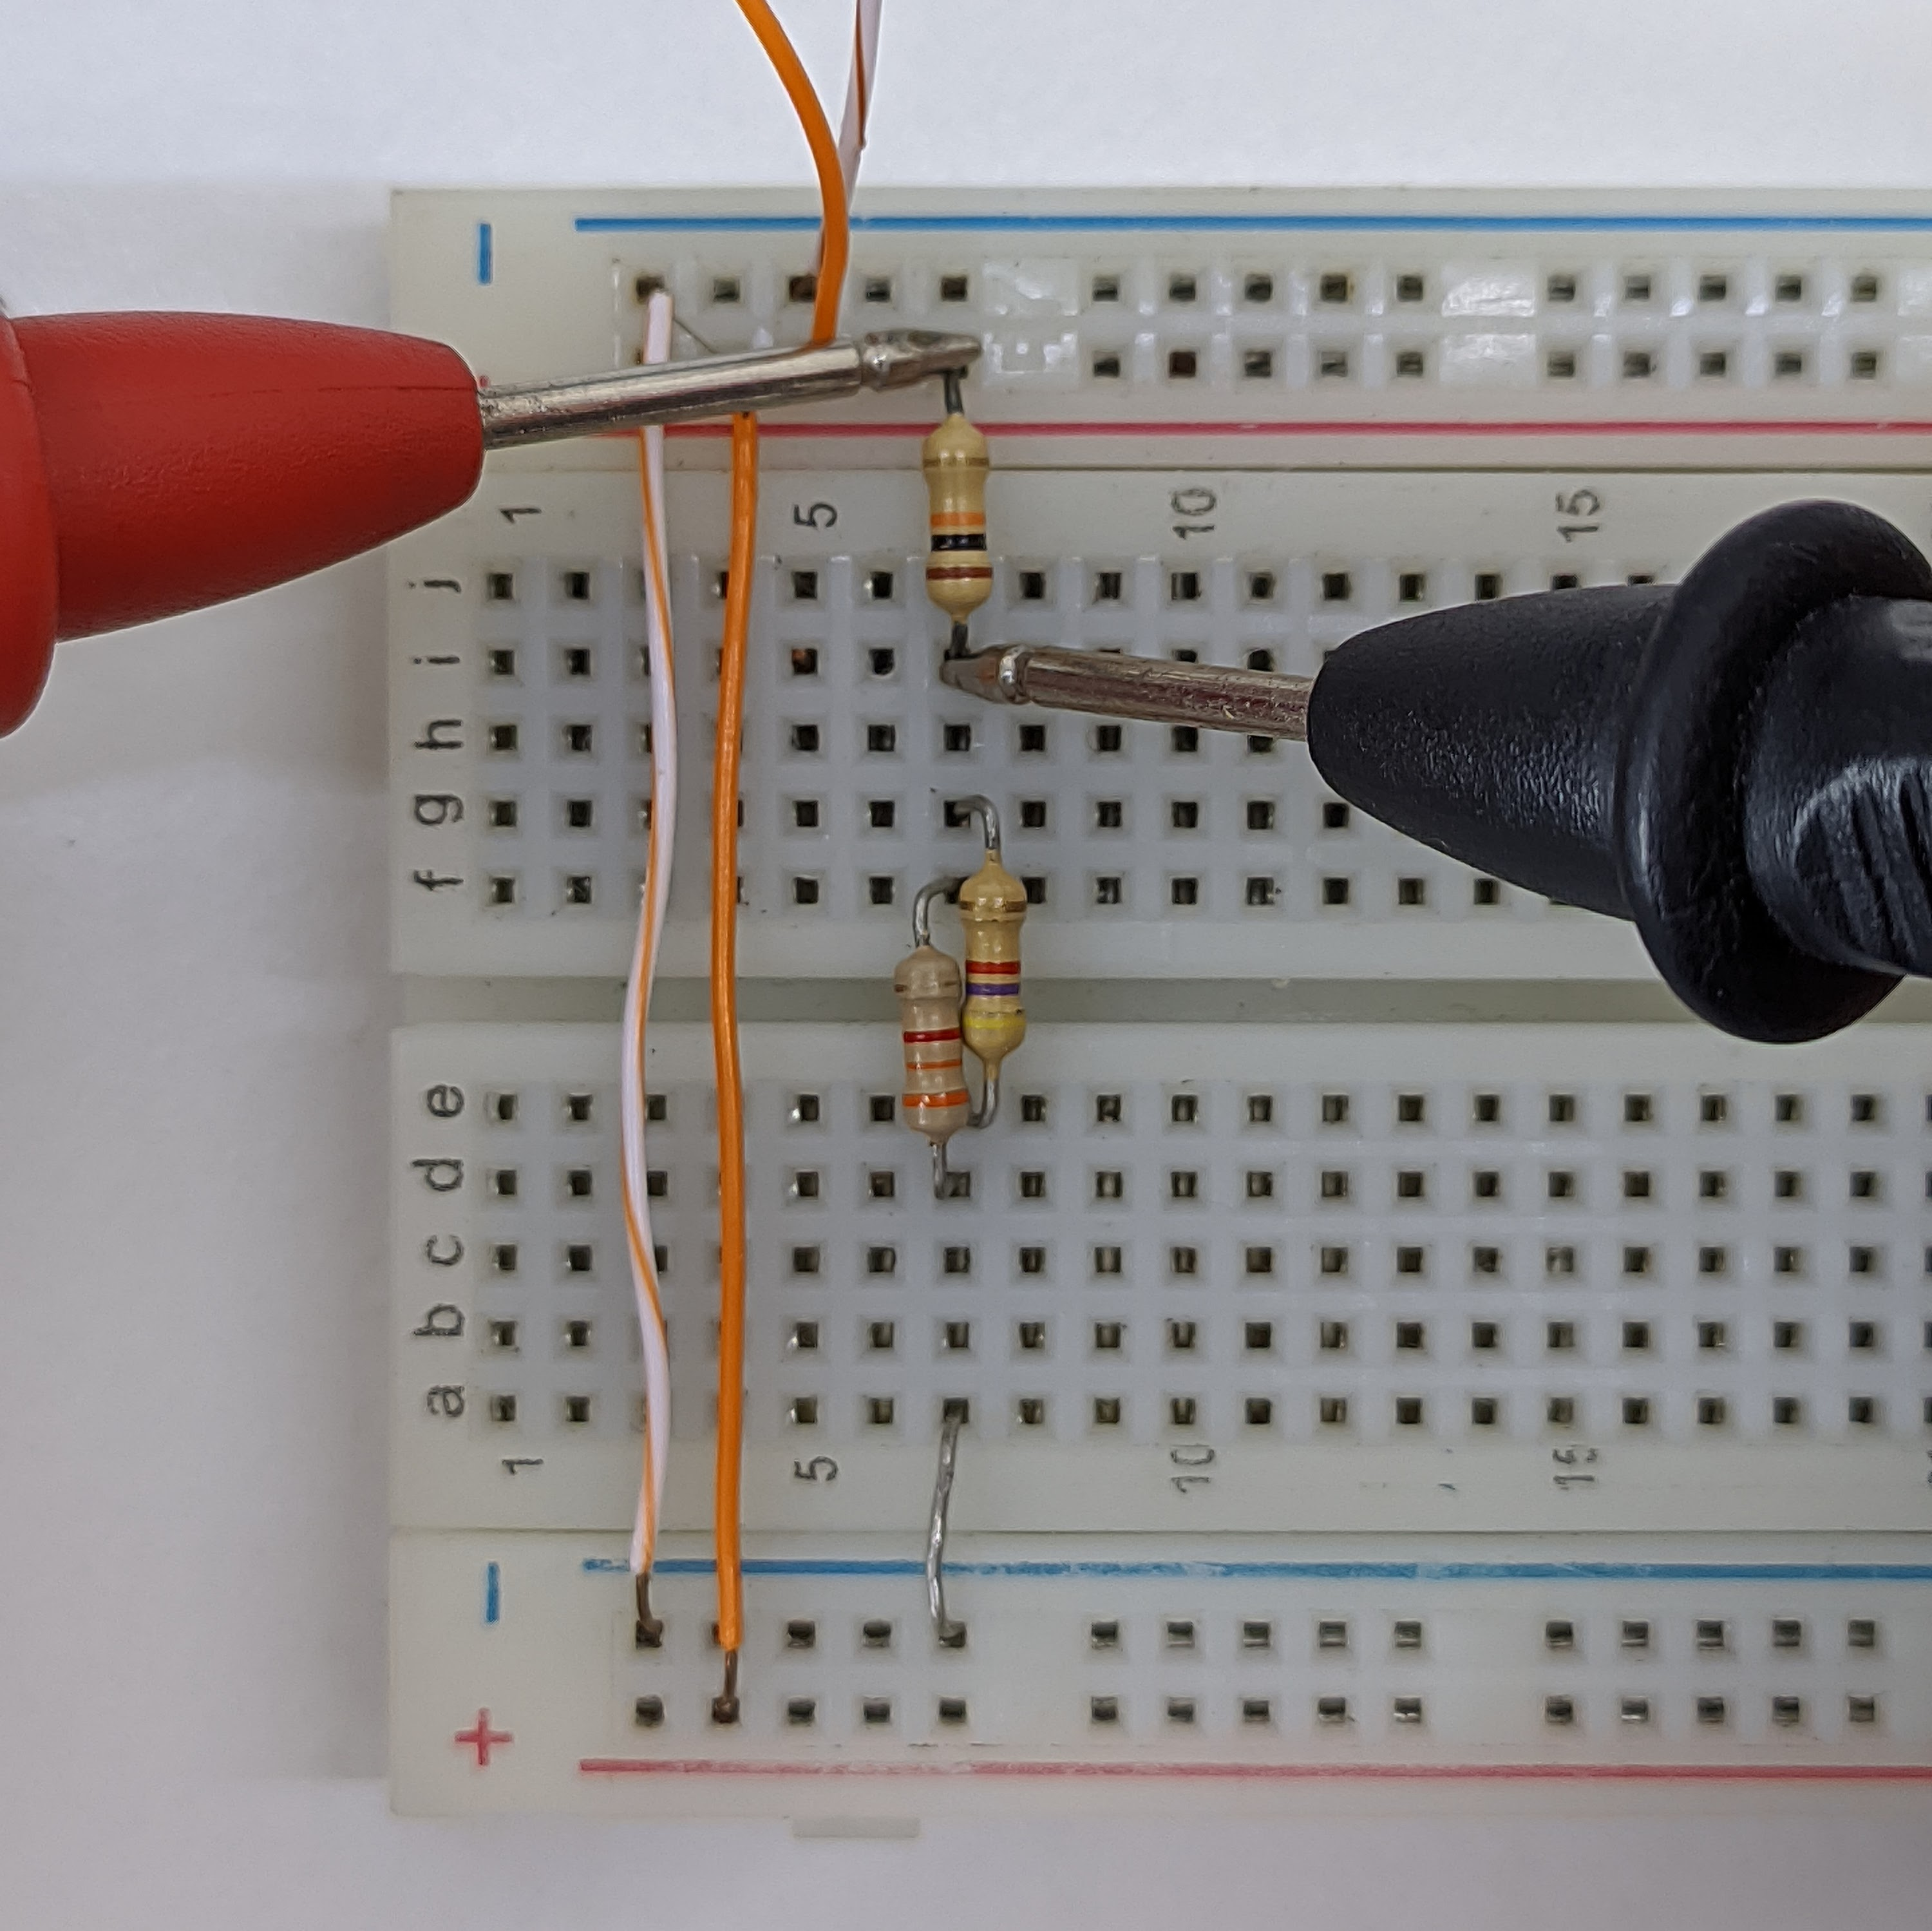
\includegraphics[width=1\linewidth]{pictures/prot-v_r1.jpg}
            \caption{Medición $V_{R_1}$.}
          \end{minipage}
          \begin{minipage}{0.3\textwidth}
            \centering
            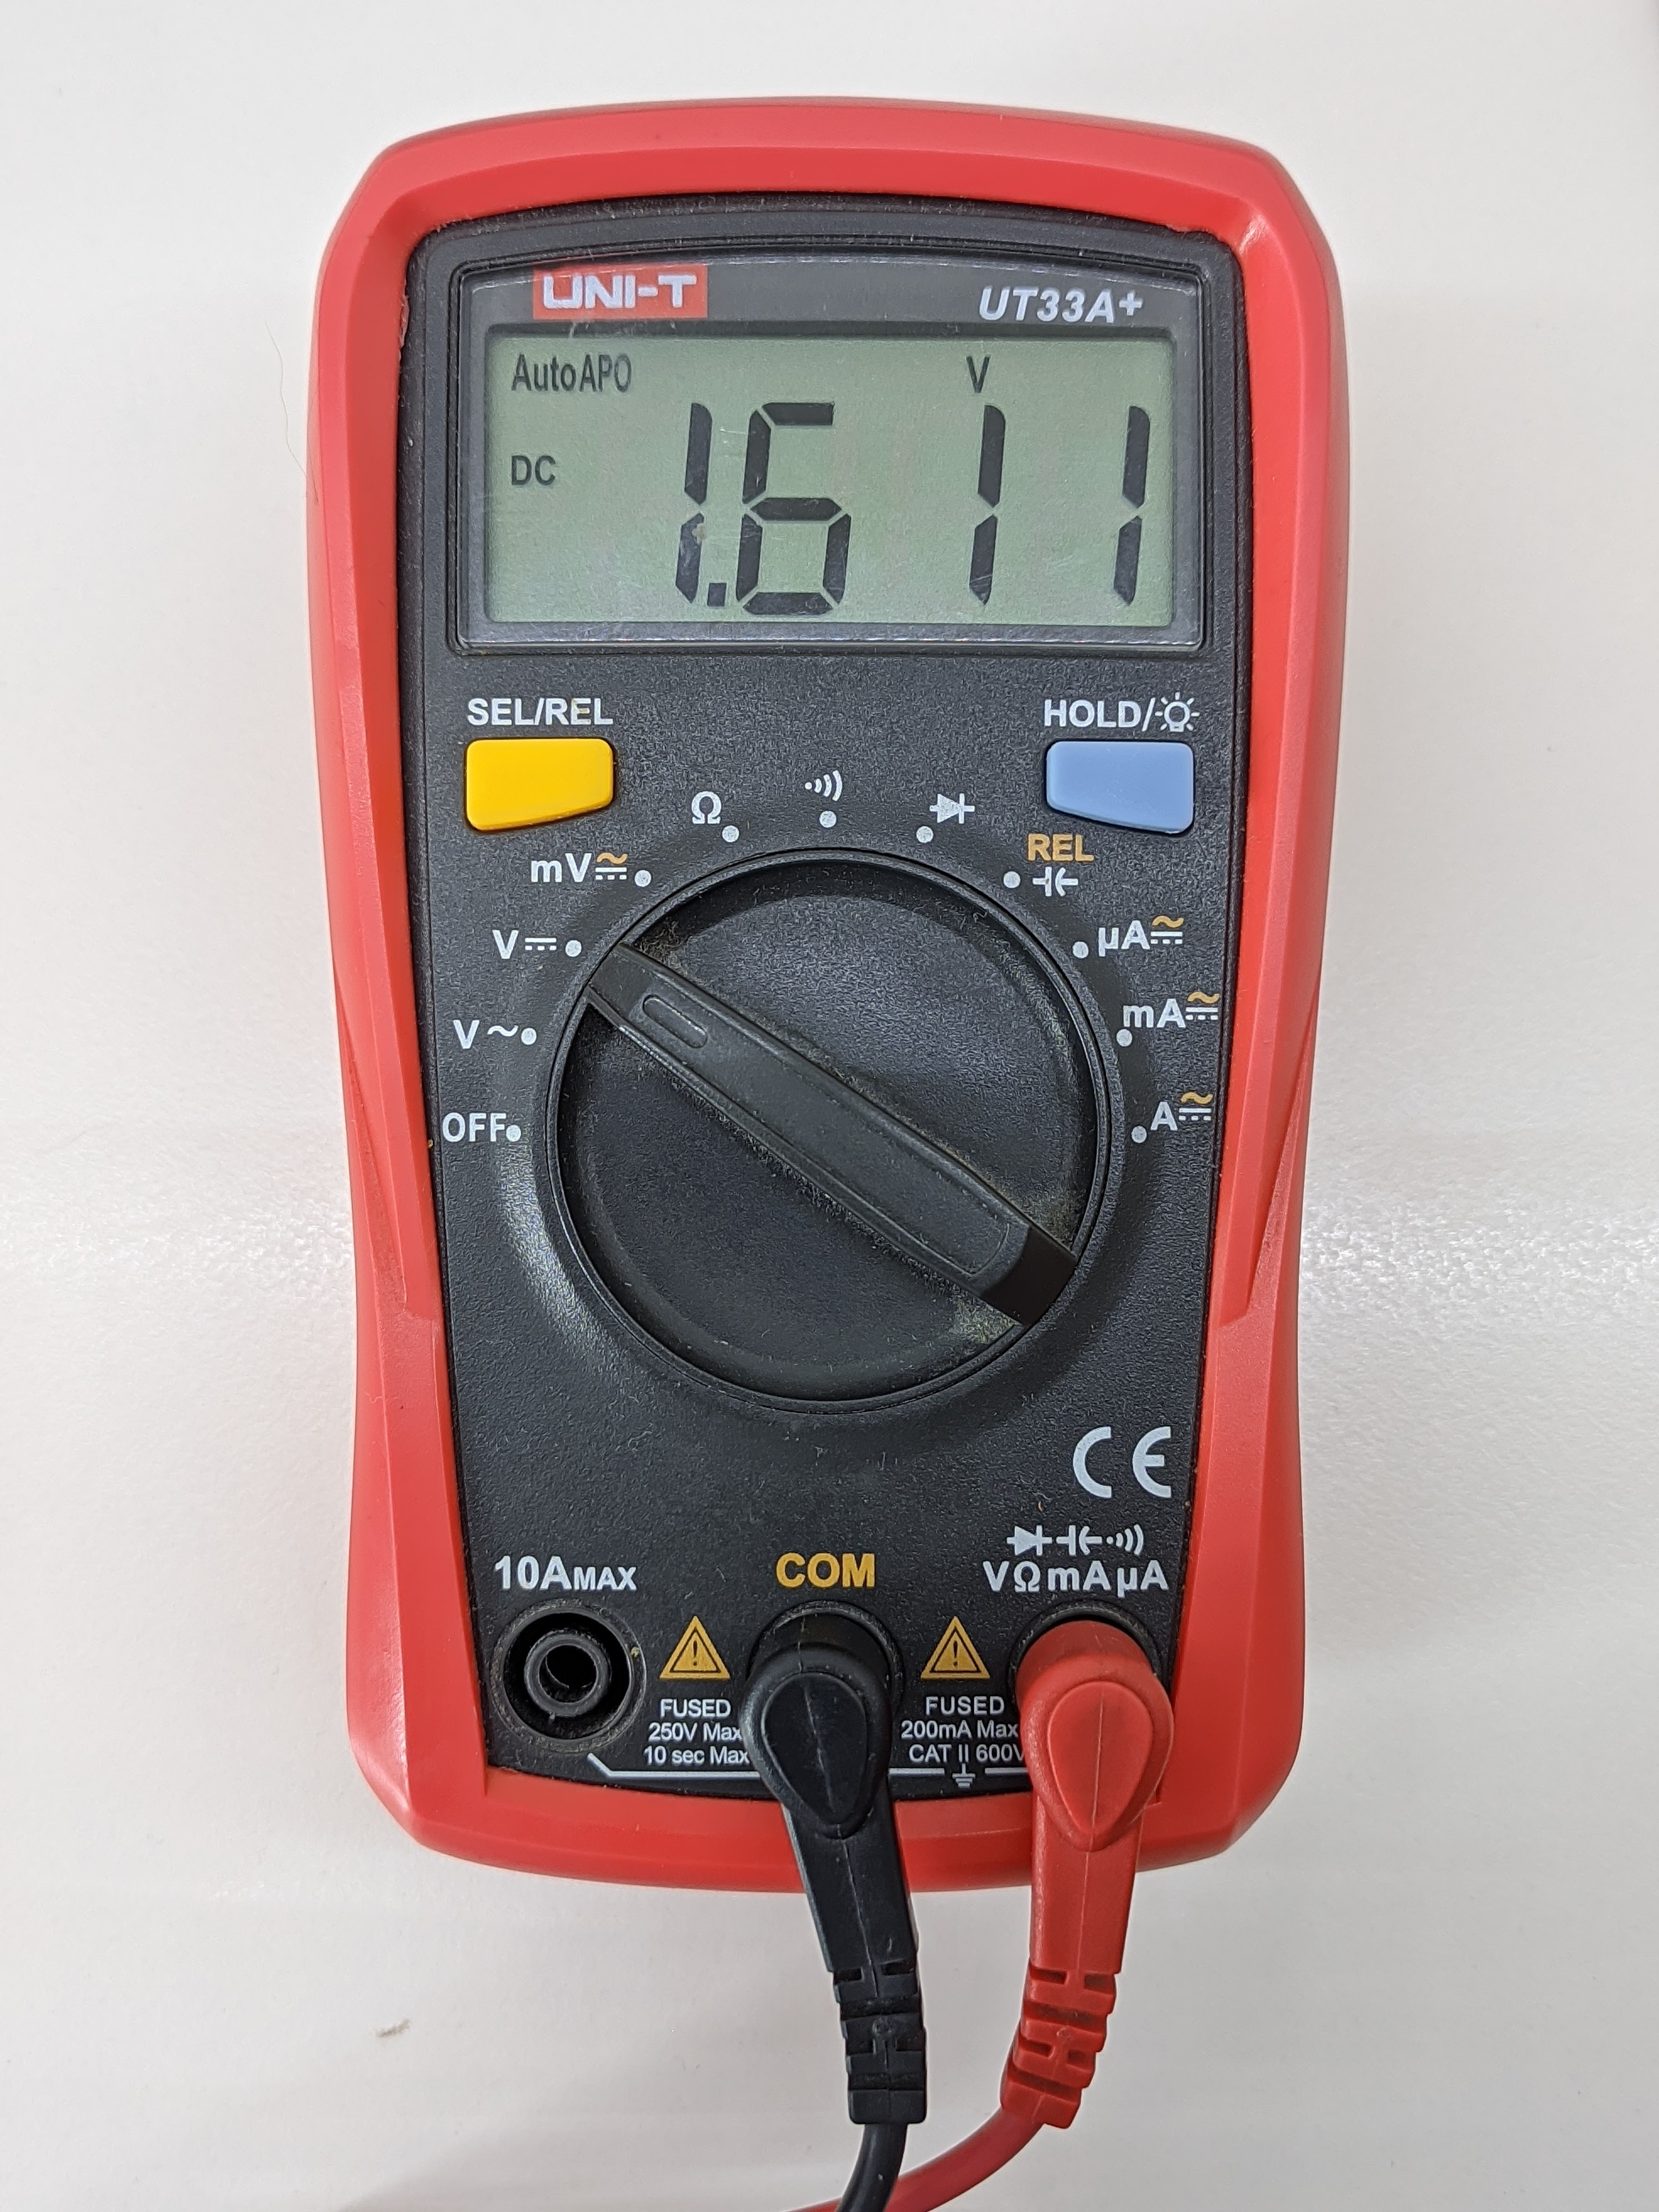
\includegraphics[width=1\linewidth]{pictures/mult-v_r2-r3.jpg}
            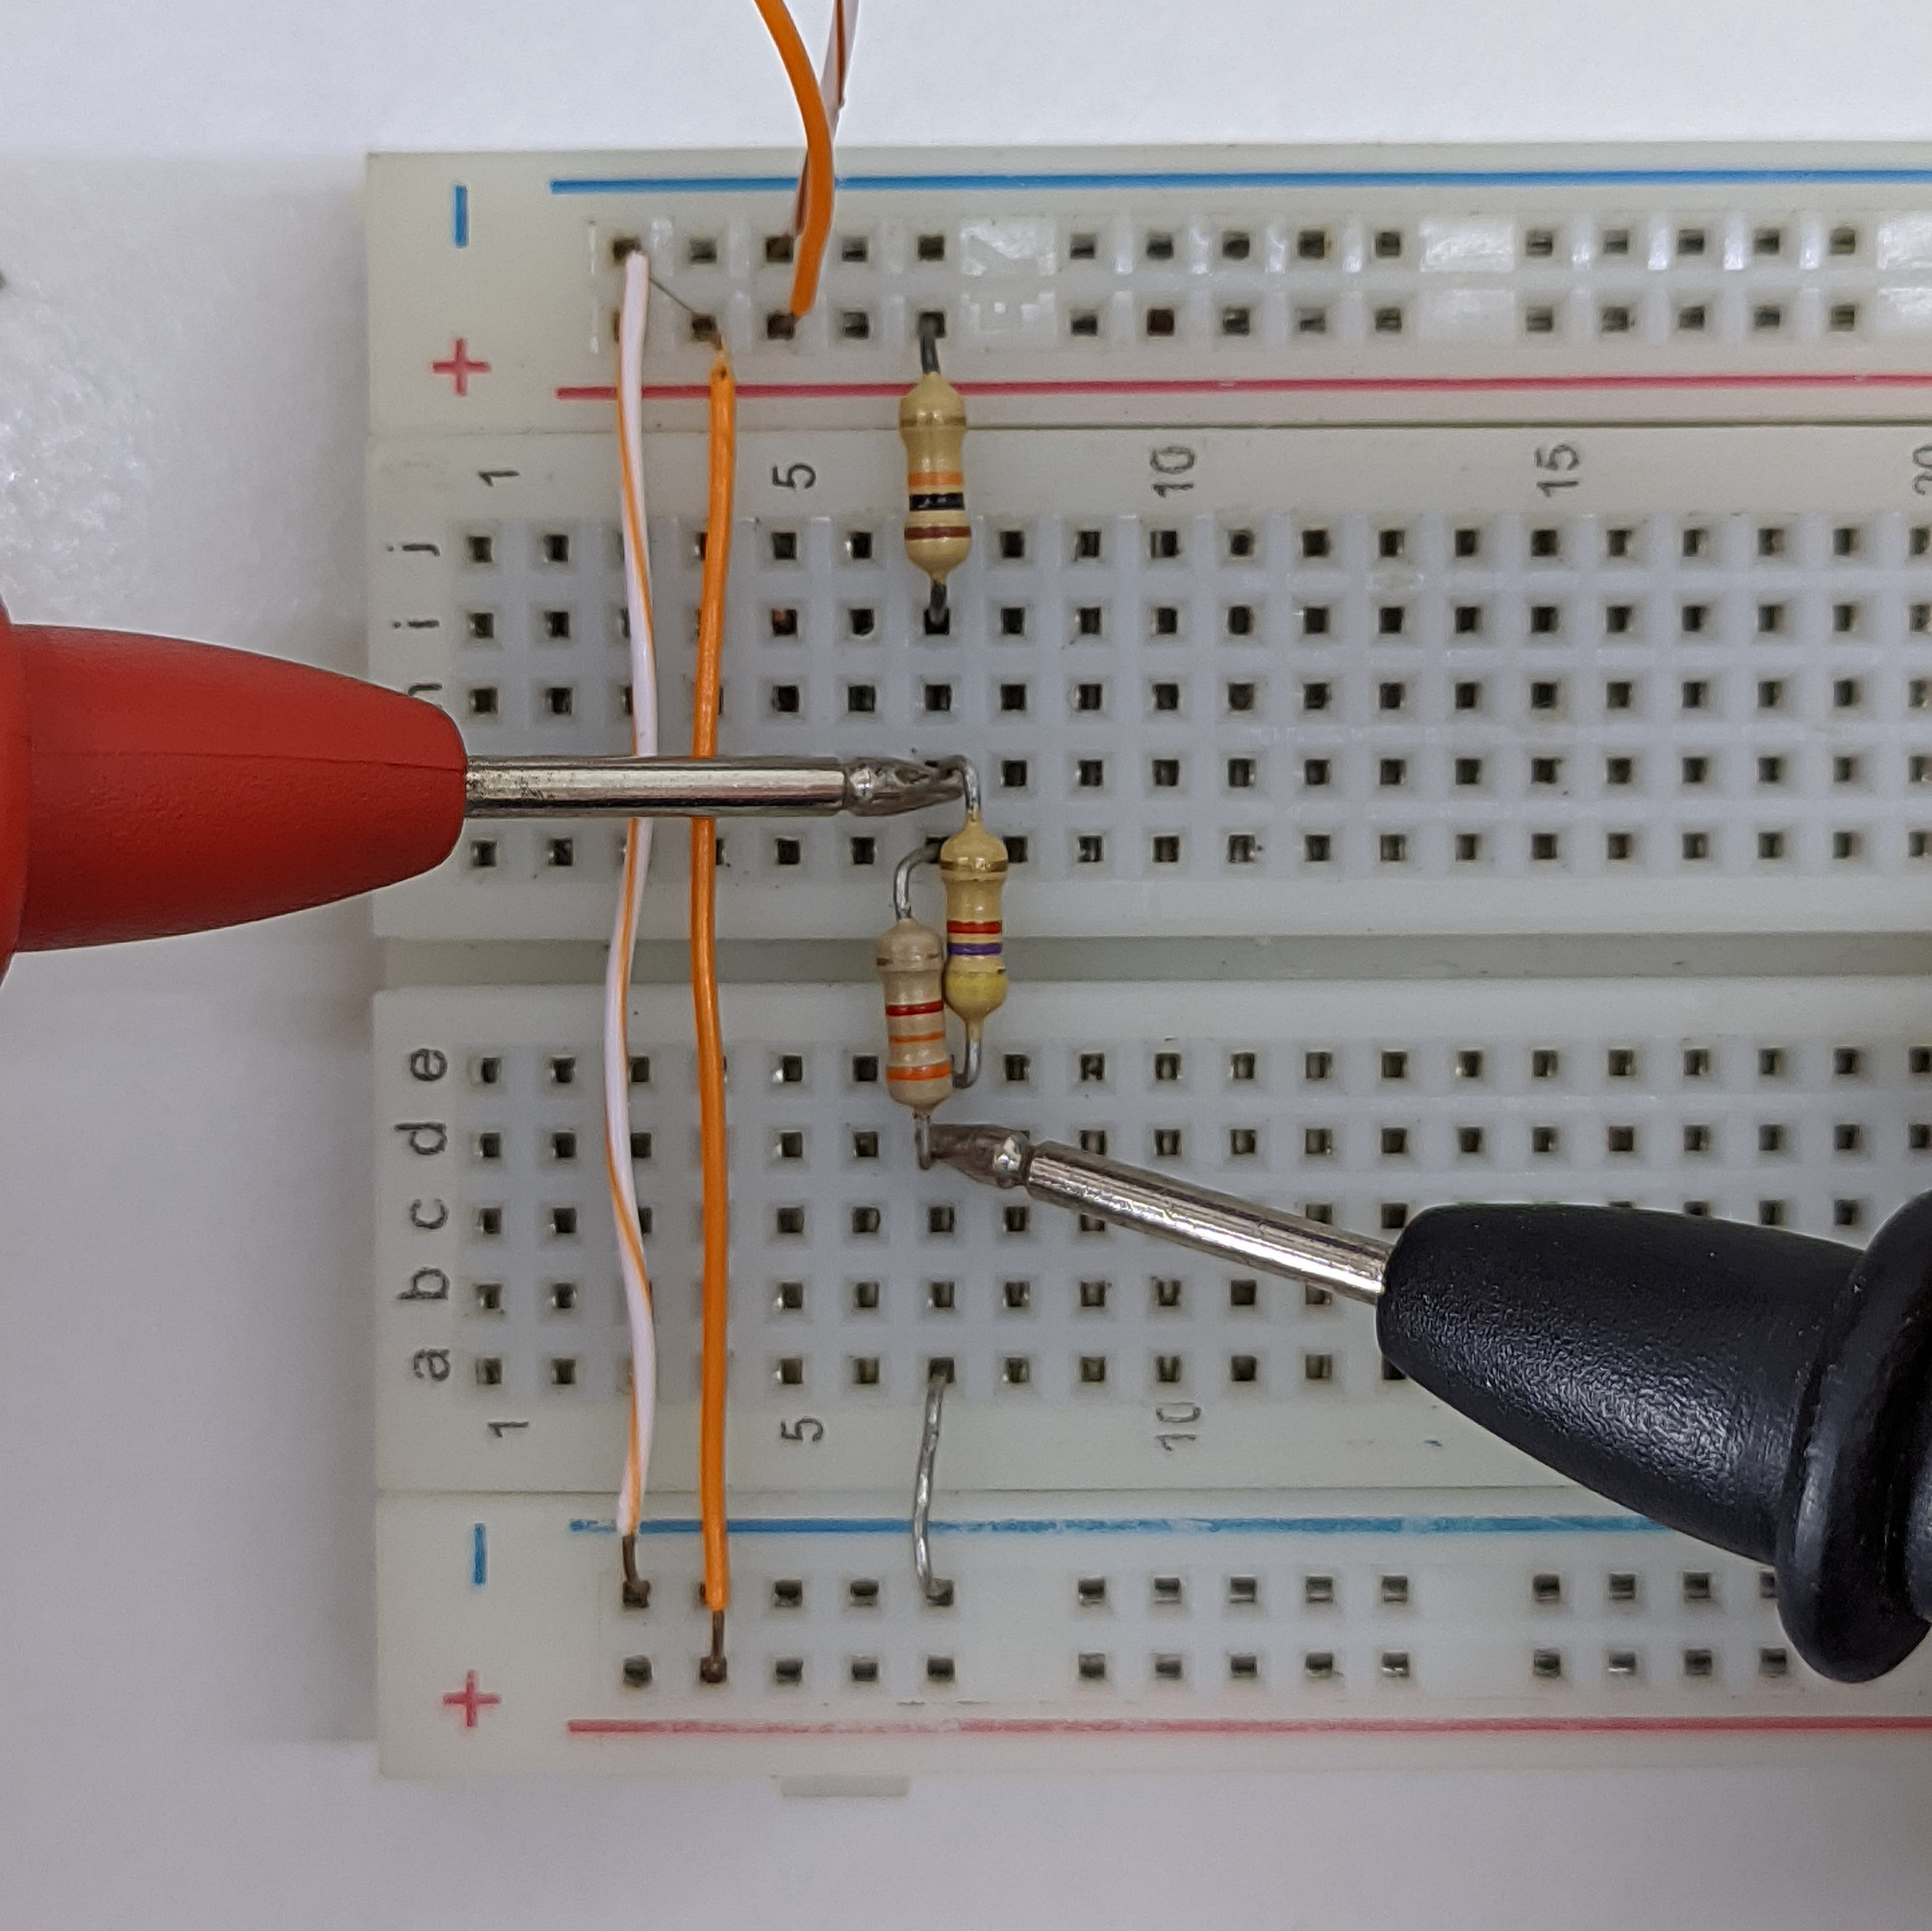
\includegraphics[width=1\linewidth]{pictures/prot-v_r2-r3.jpg}
            \caption{Medición $V_{R_2}$.}
          \end{minipage}
          \begin{minipage}{0.3\textwidth}
            \centering
            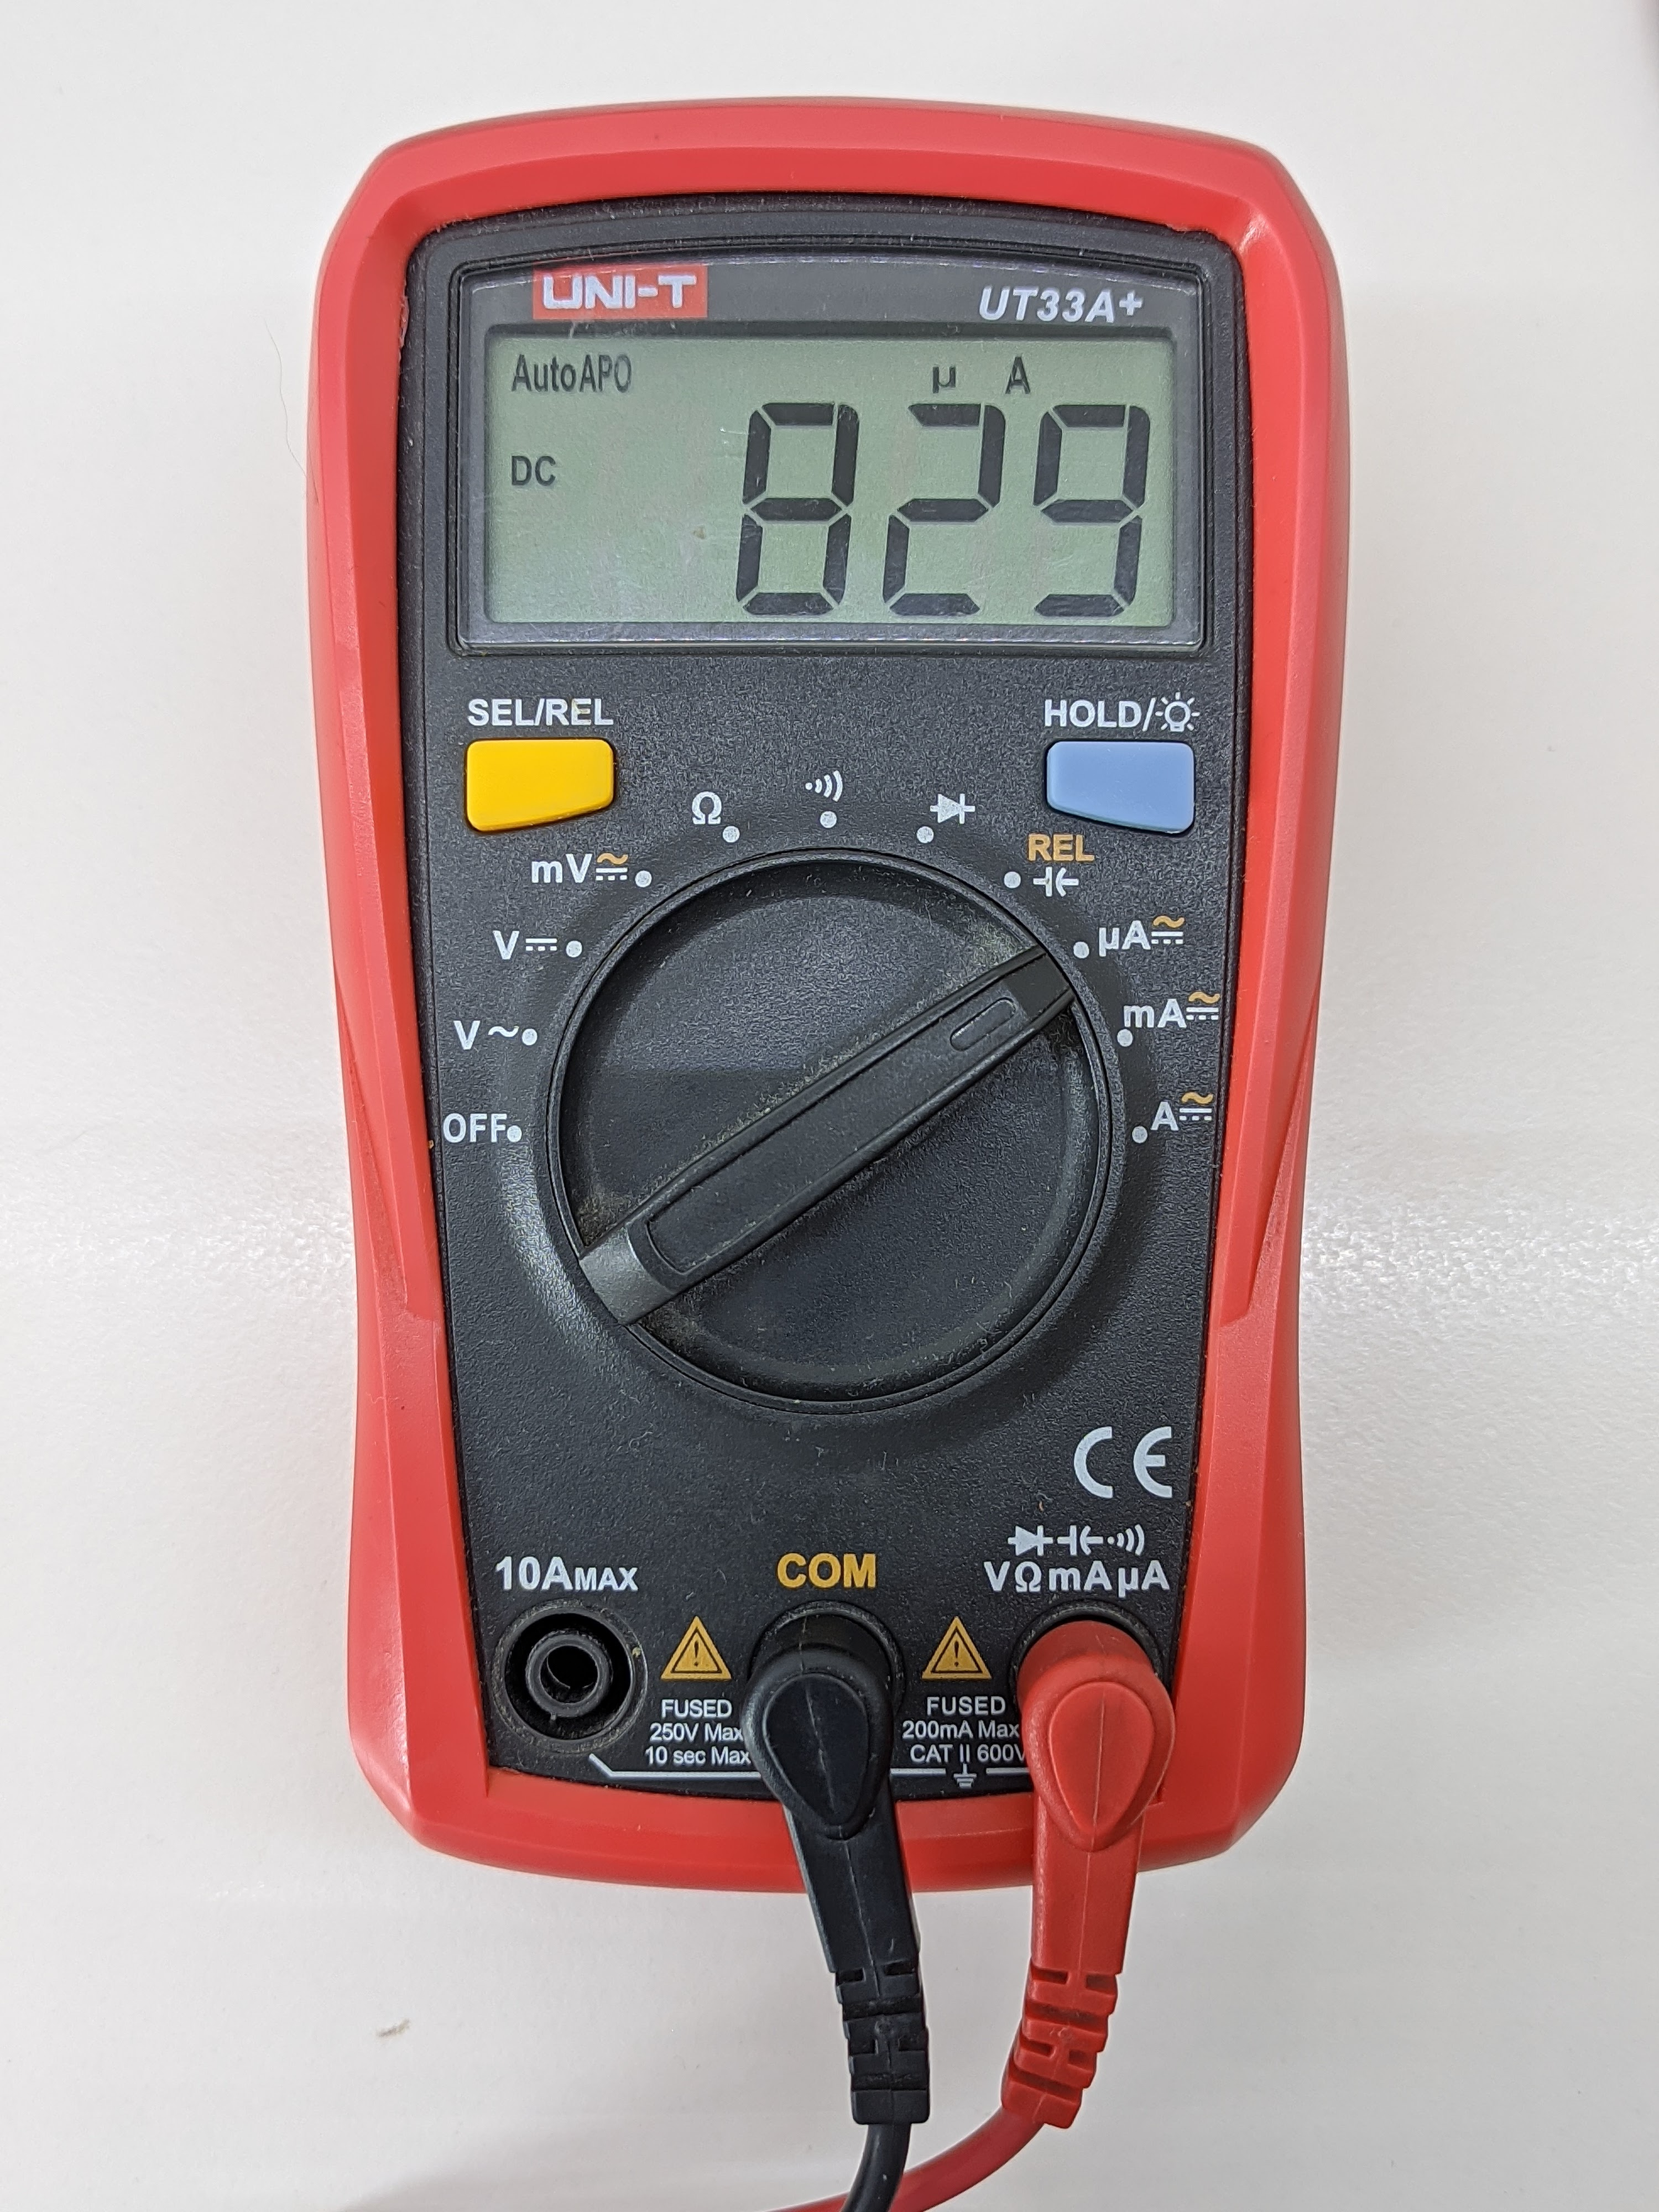
\includegraphics[width=1\linewidth]{pictures/mult-it.jpg}
            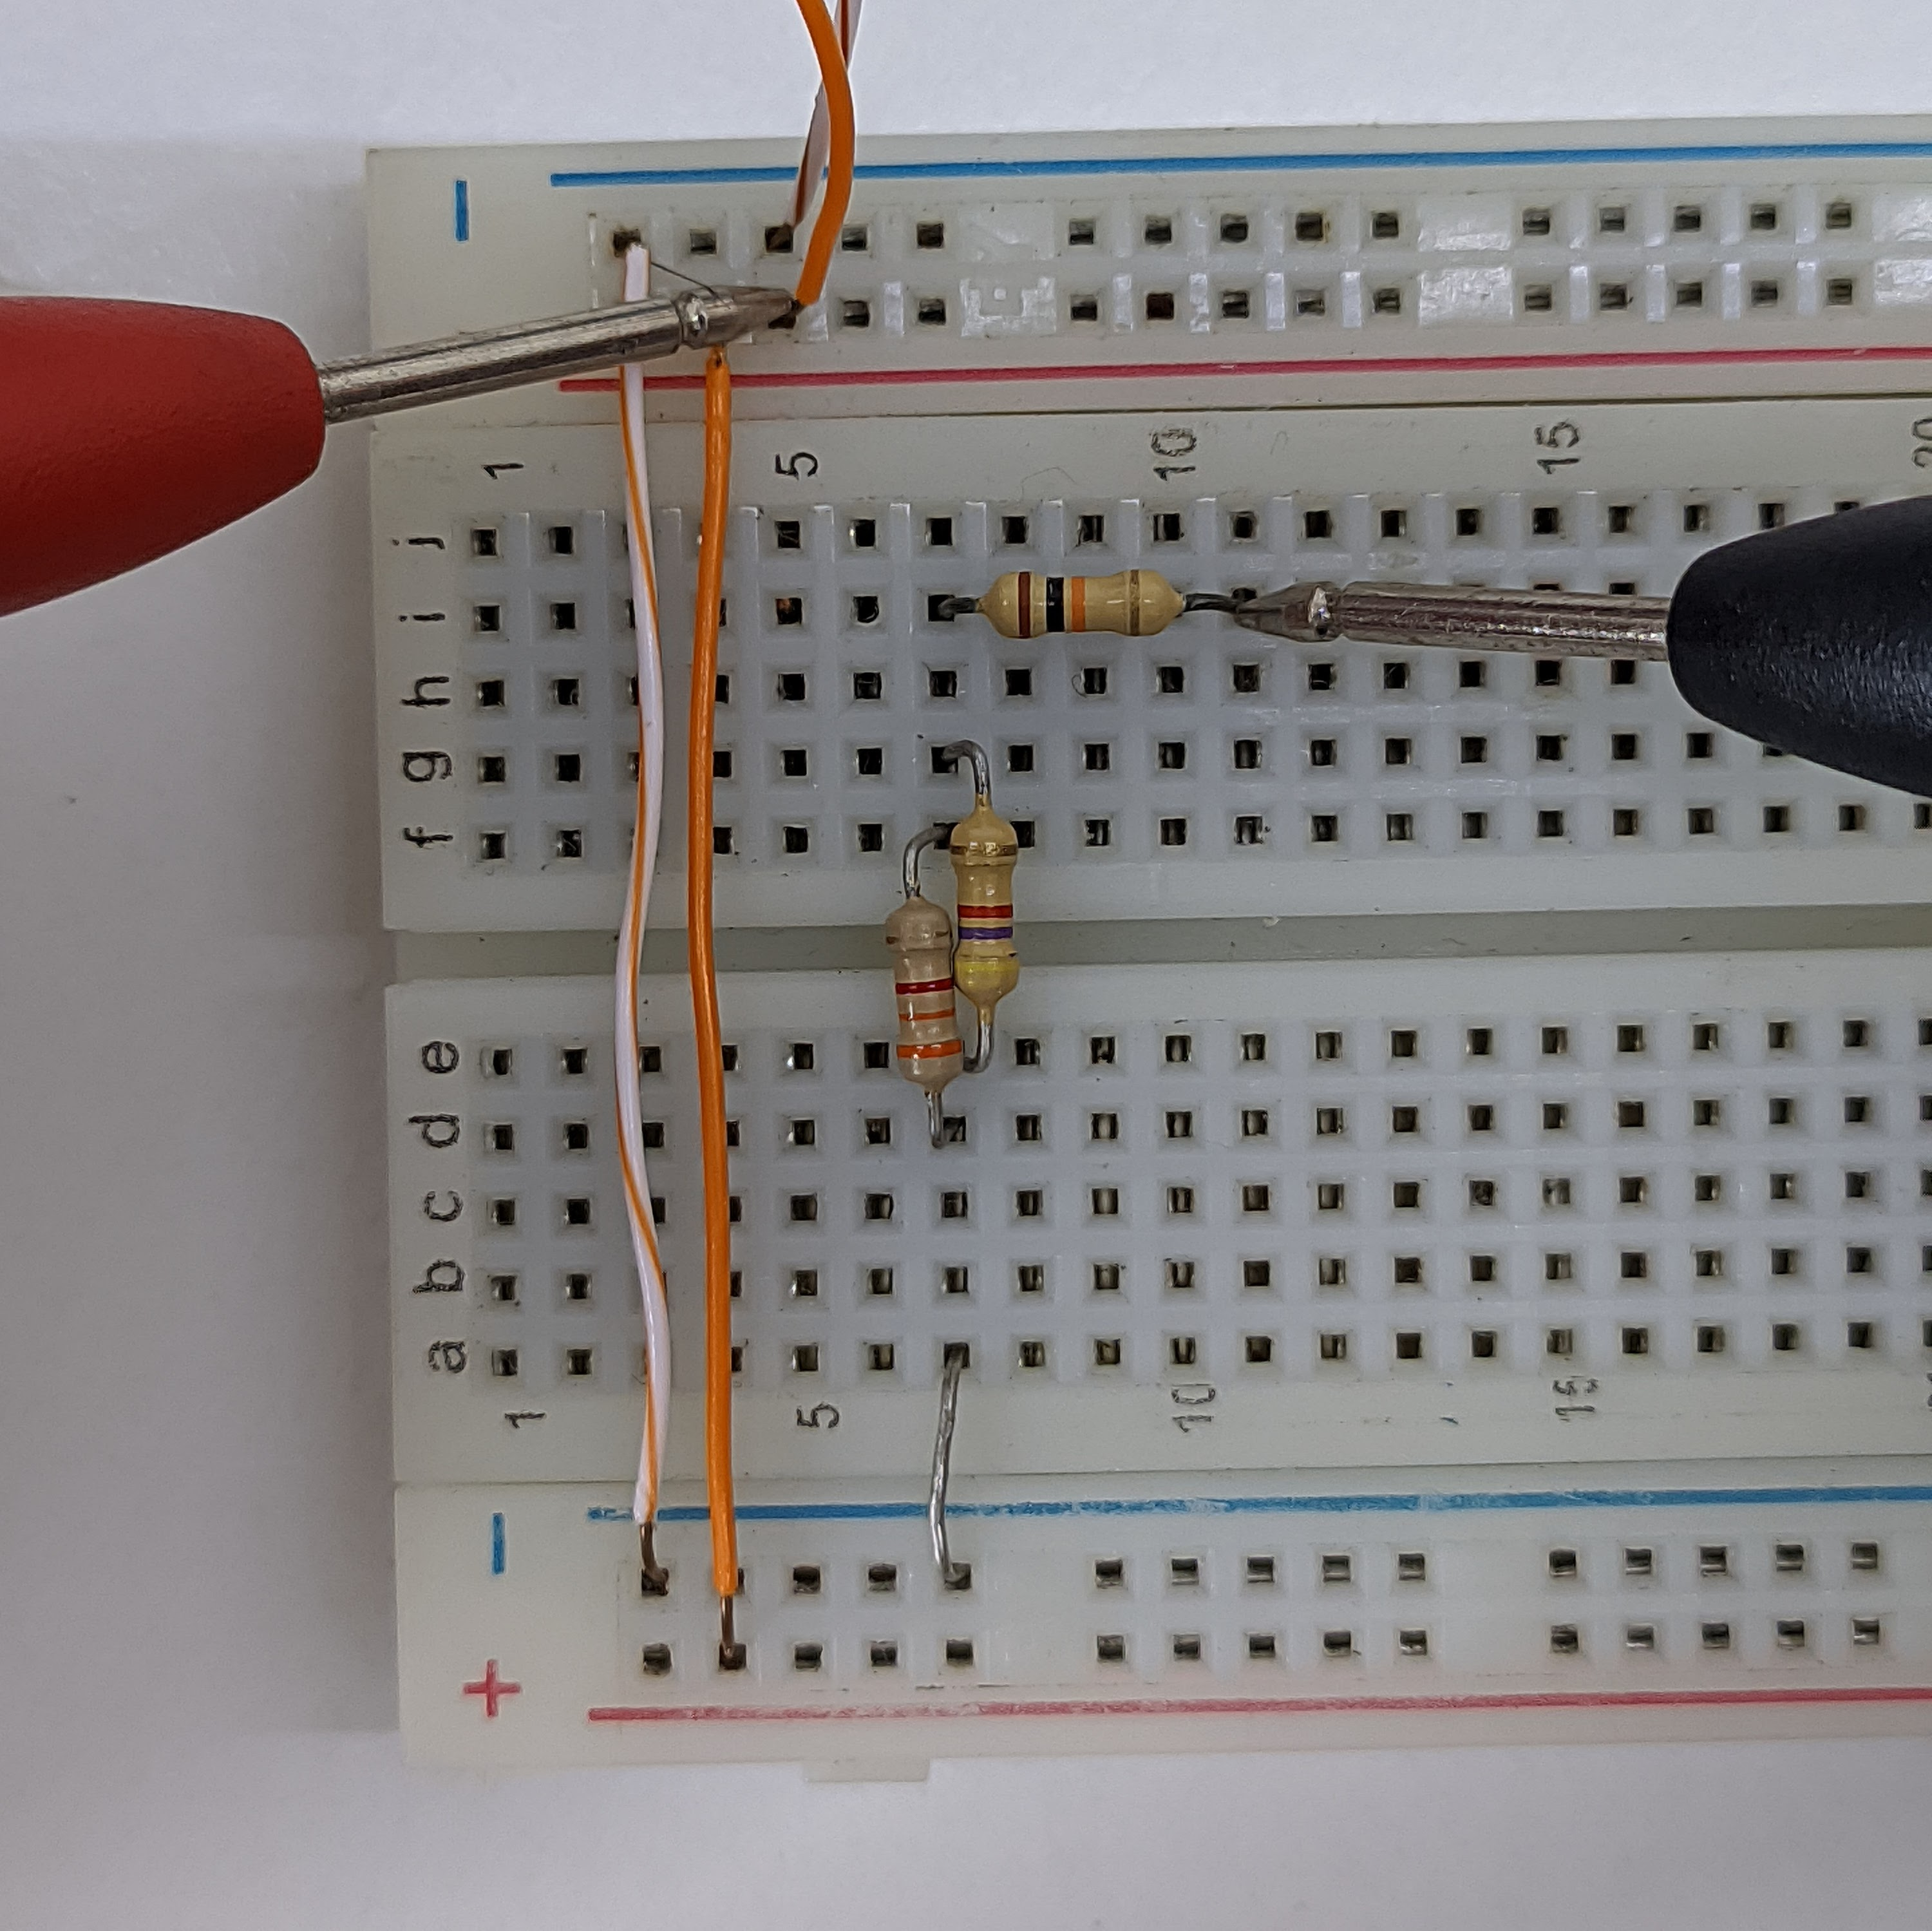
\includegraphics[width=1\linewidth]{pictures/prot-it.jpg}
            \caption{Medición $I_t$.}
          \end{minipage}
      \end{figure}
      \vspace{-0.5cm}
      \begin{figure}[H]
        \centering
          \begin{minipage}{0.3\textwidth}
            \centering
            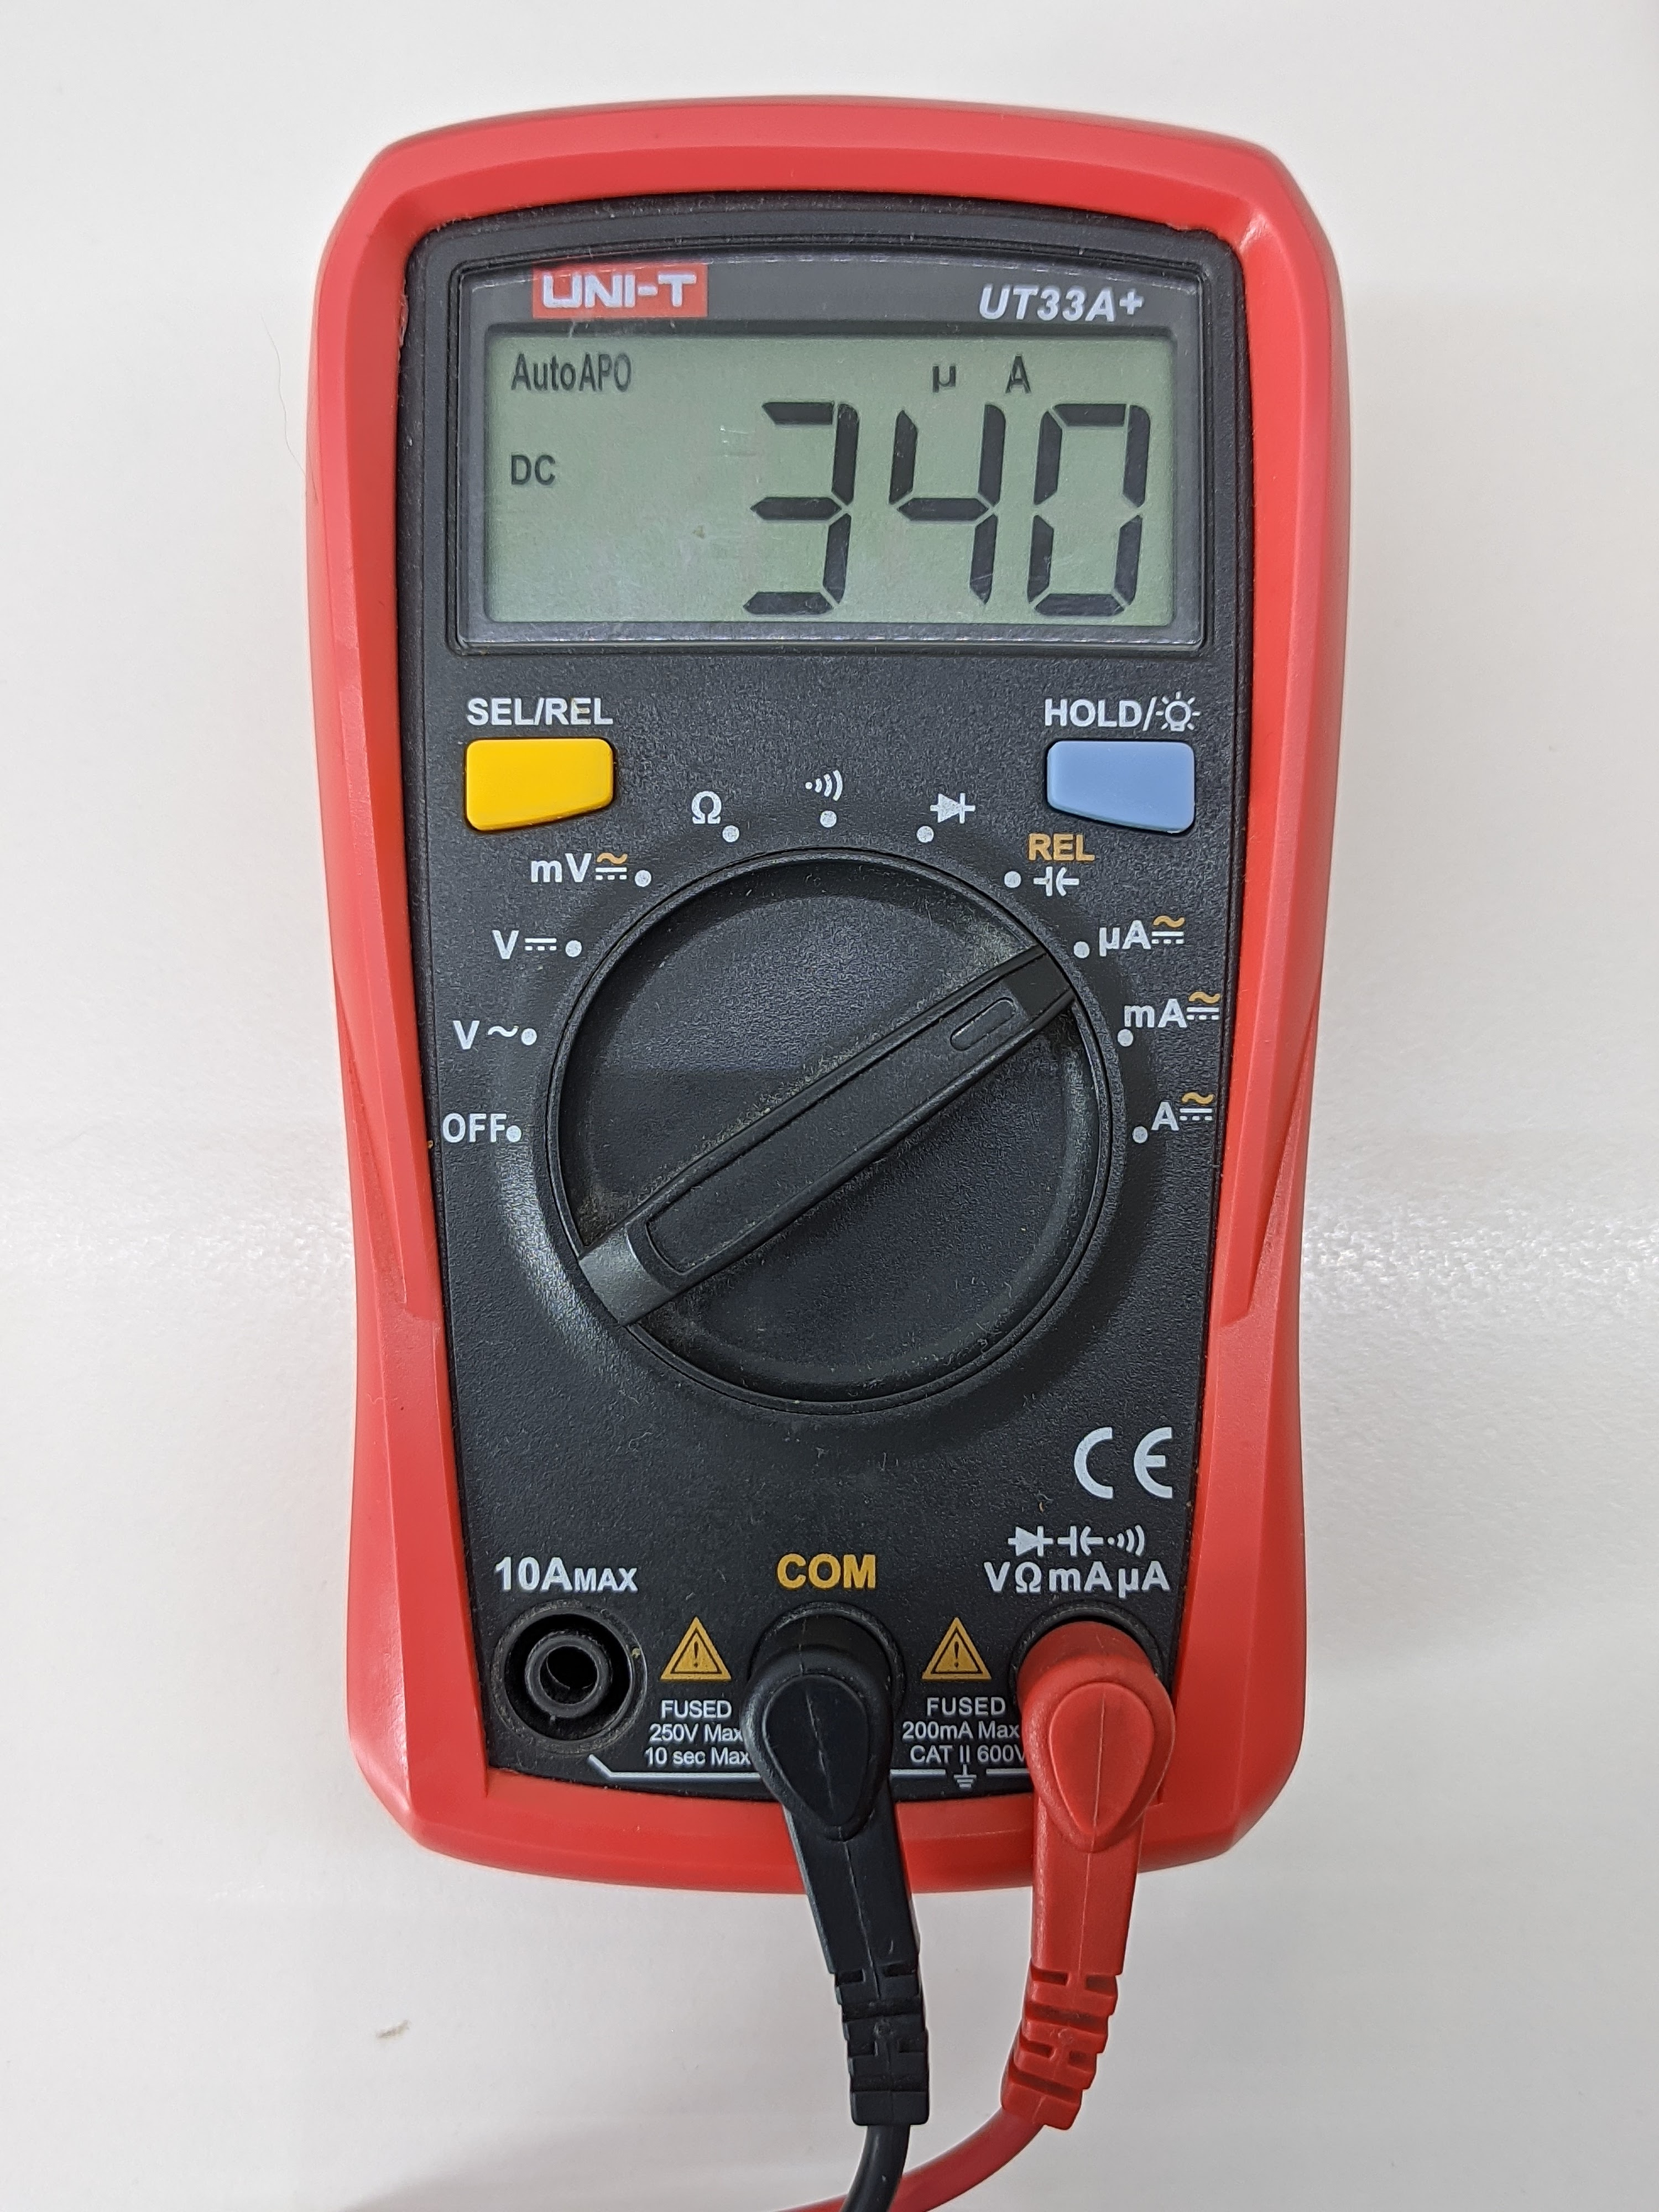
\includegraphics[width=1\linewidth]{pictures/mult-i2.jpg}
            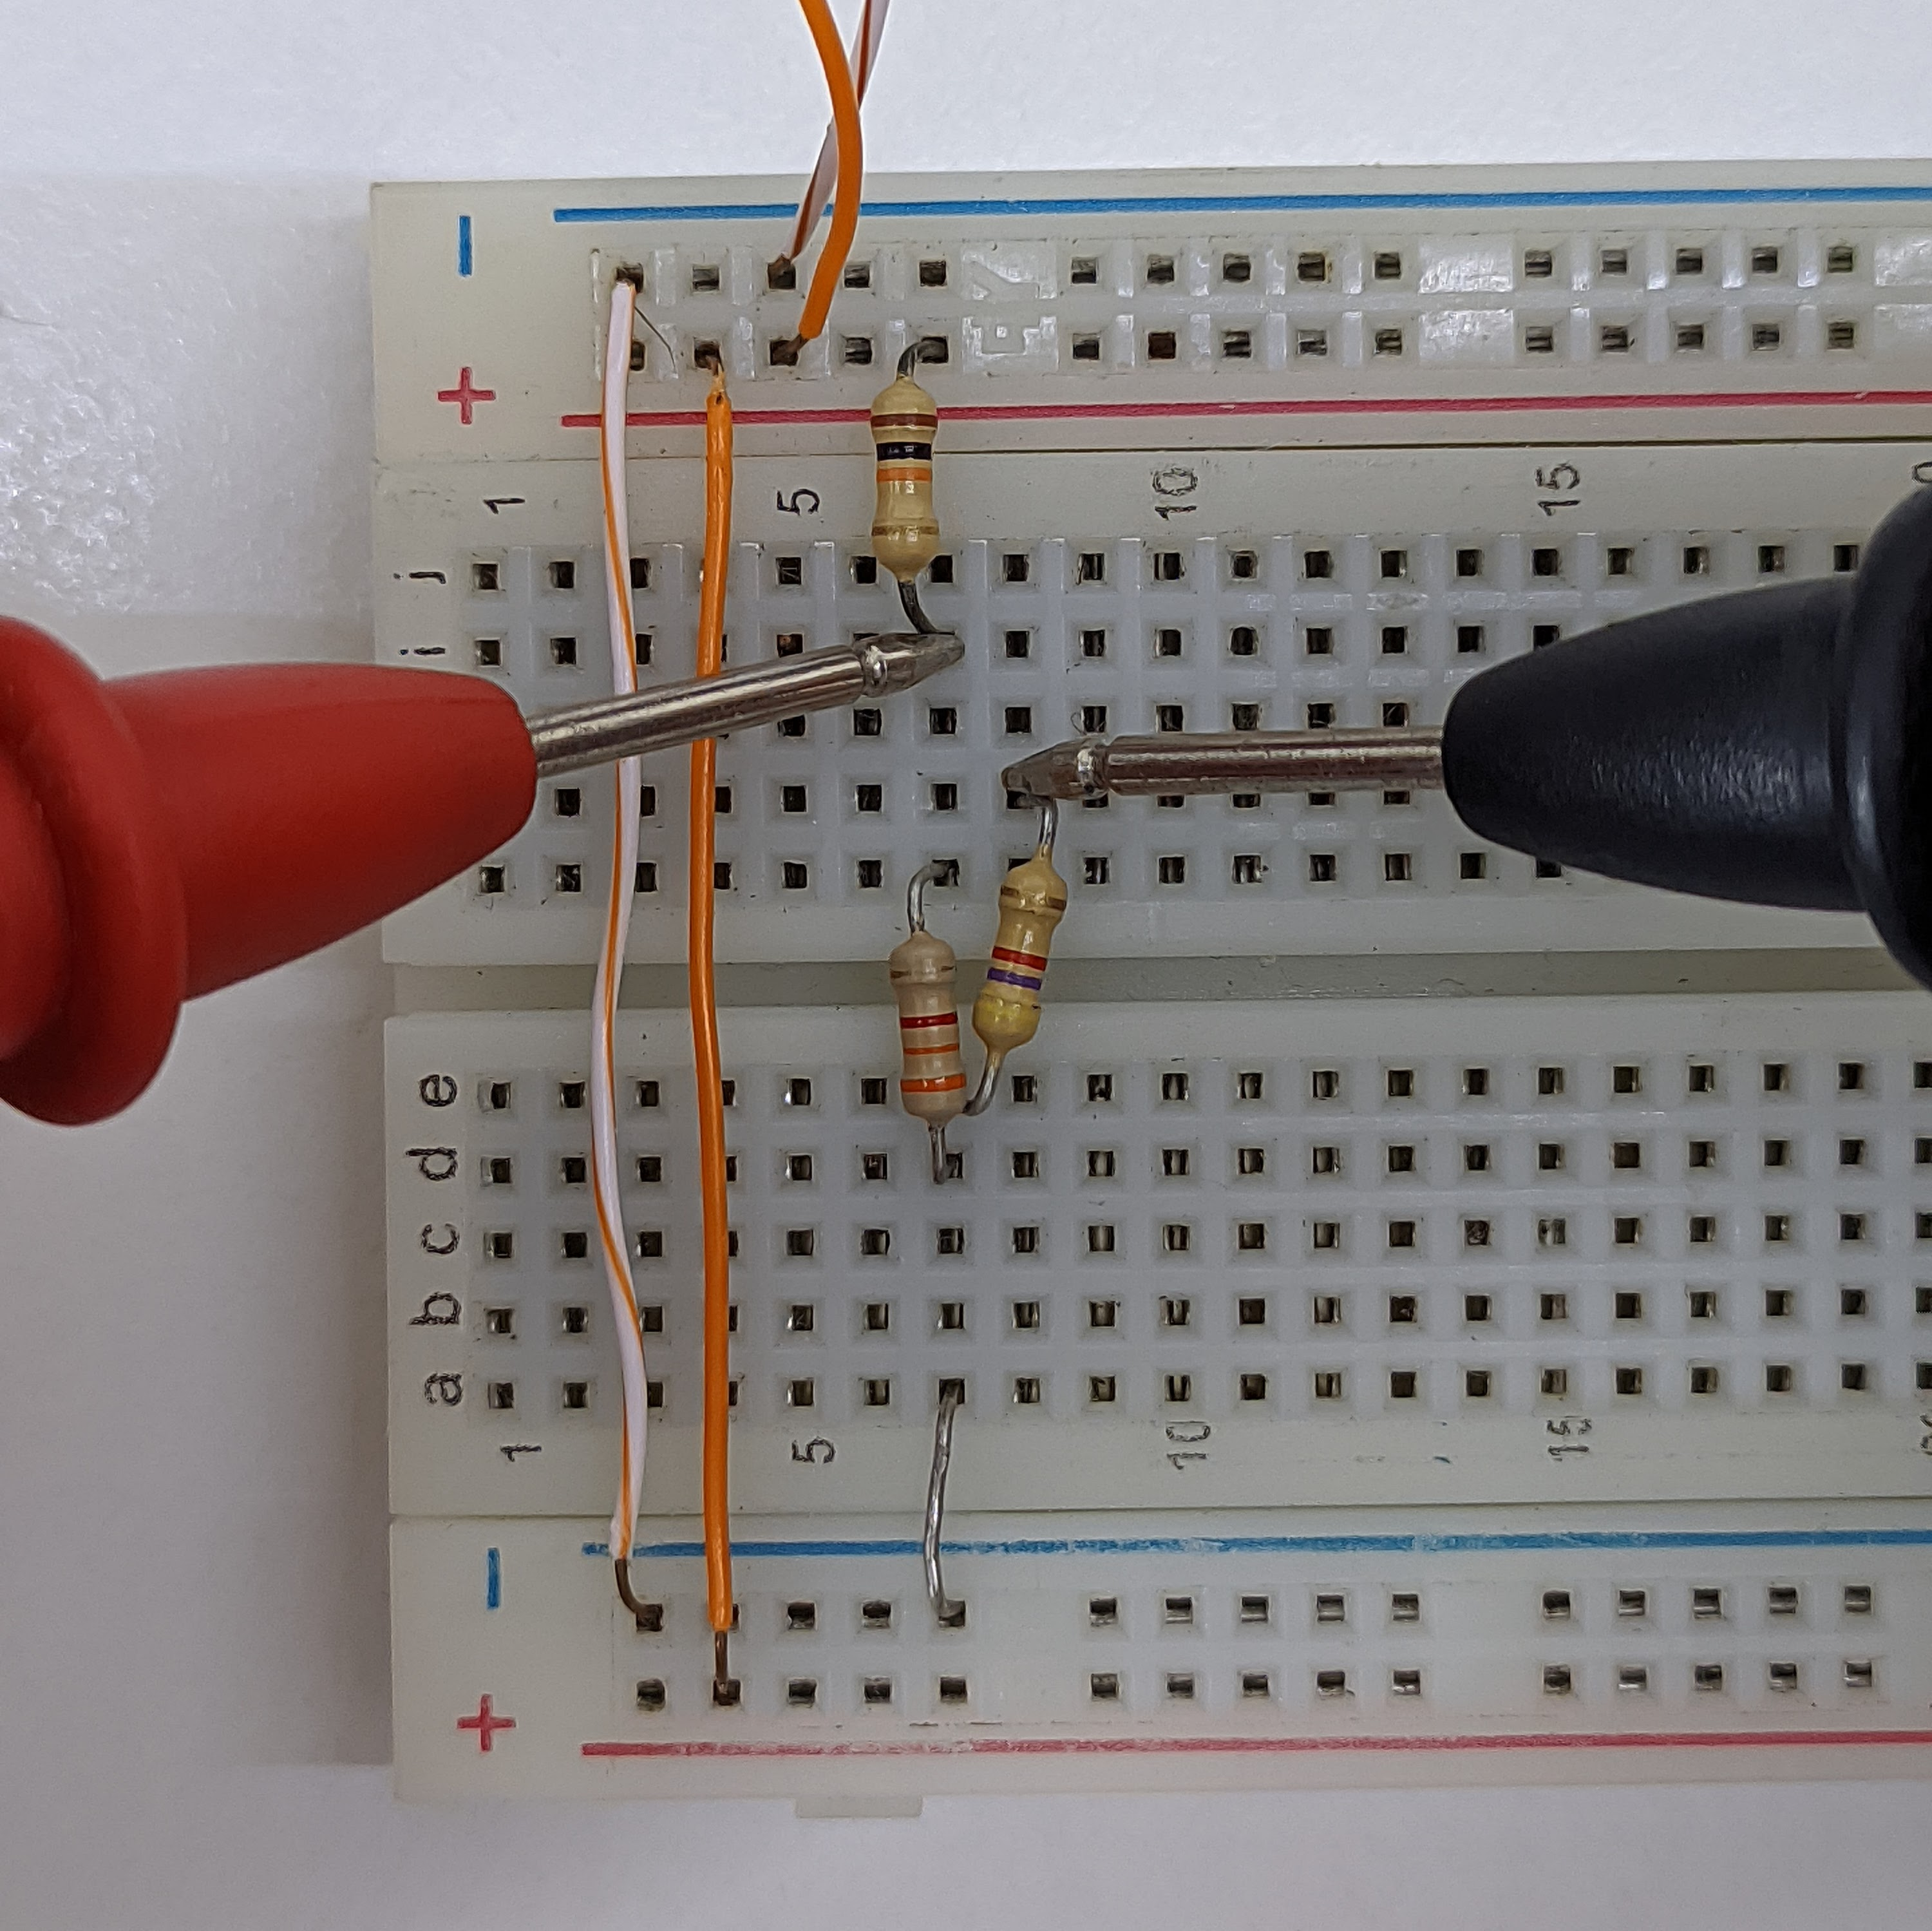
\includegraphics[width=1\linewidth]{pictures/prot-i2.jpg}
            \caption{Medición $I_2$.}
          \end{minipage}
          \begin{minipage}{0.3\textwidth}
            \centering
            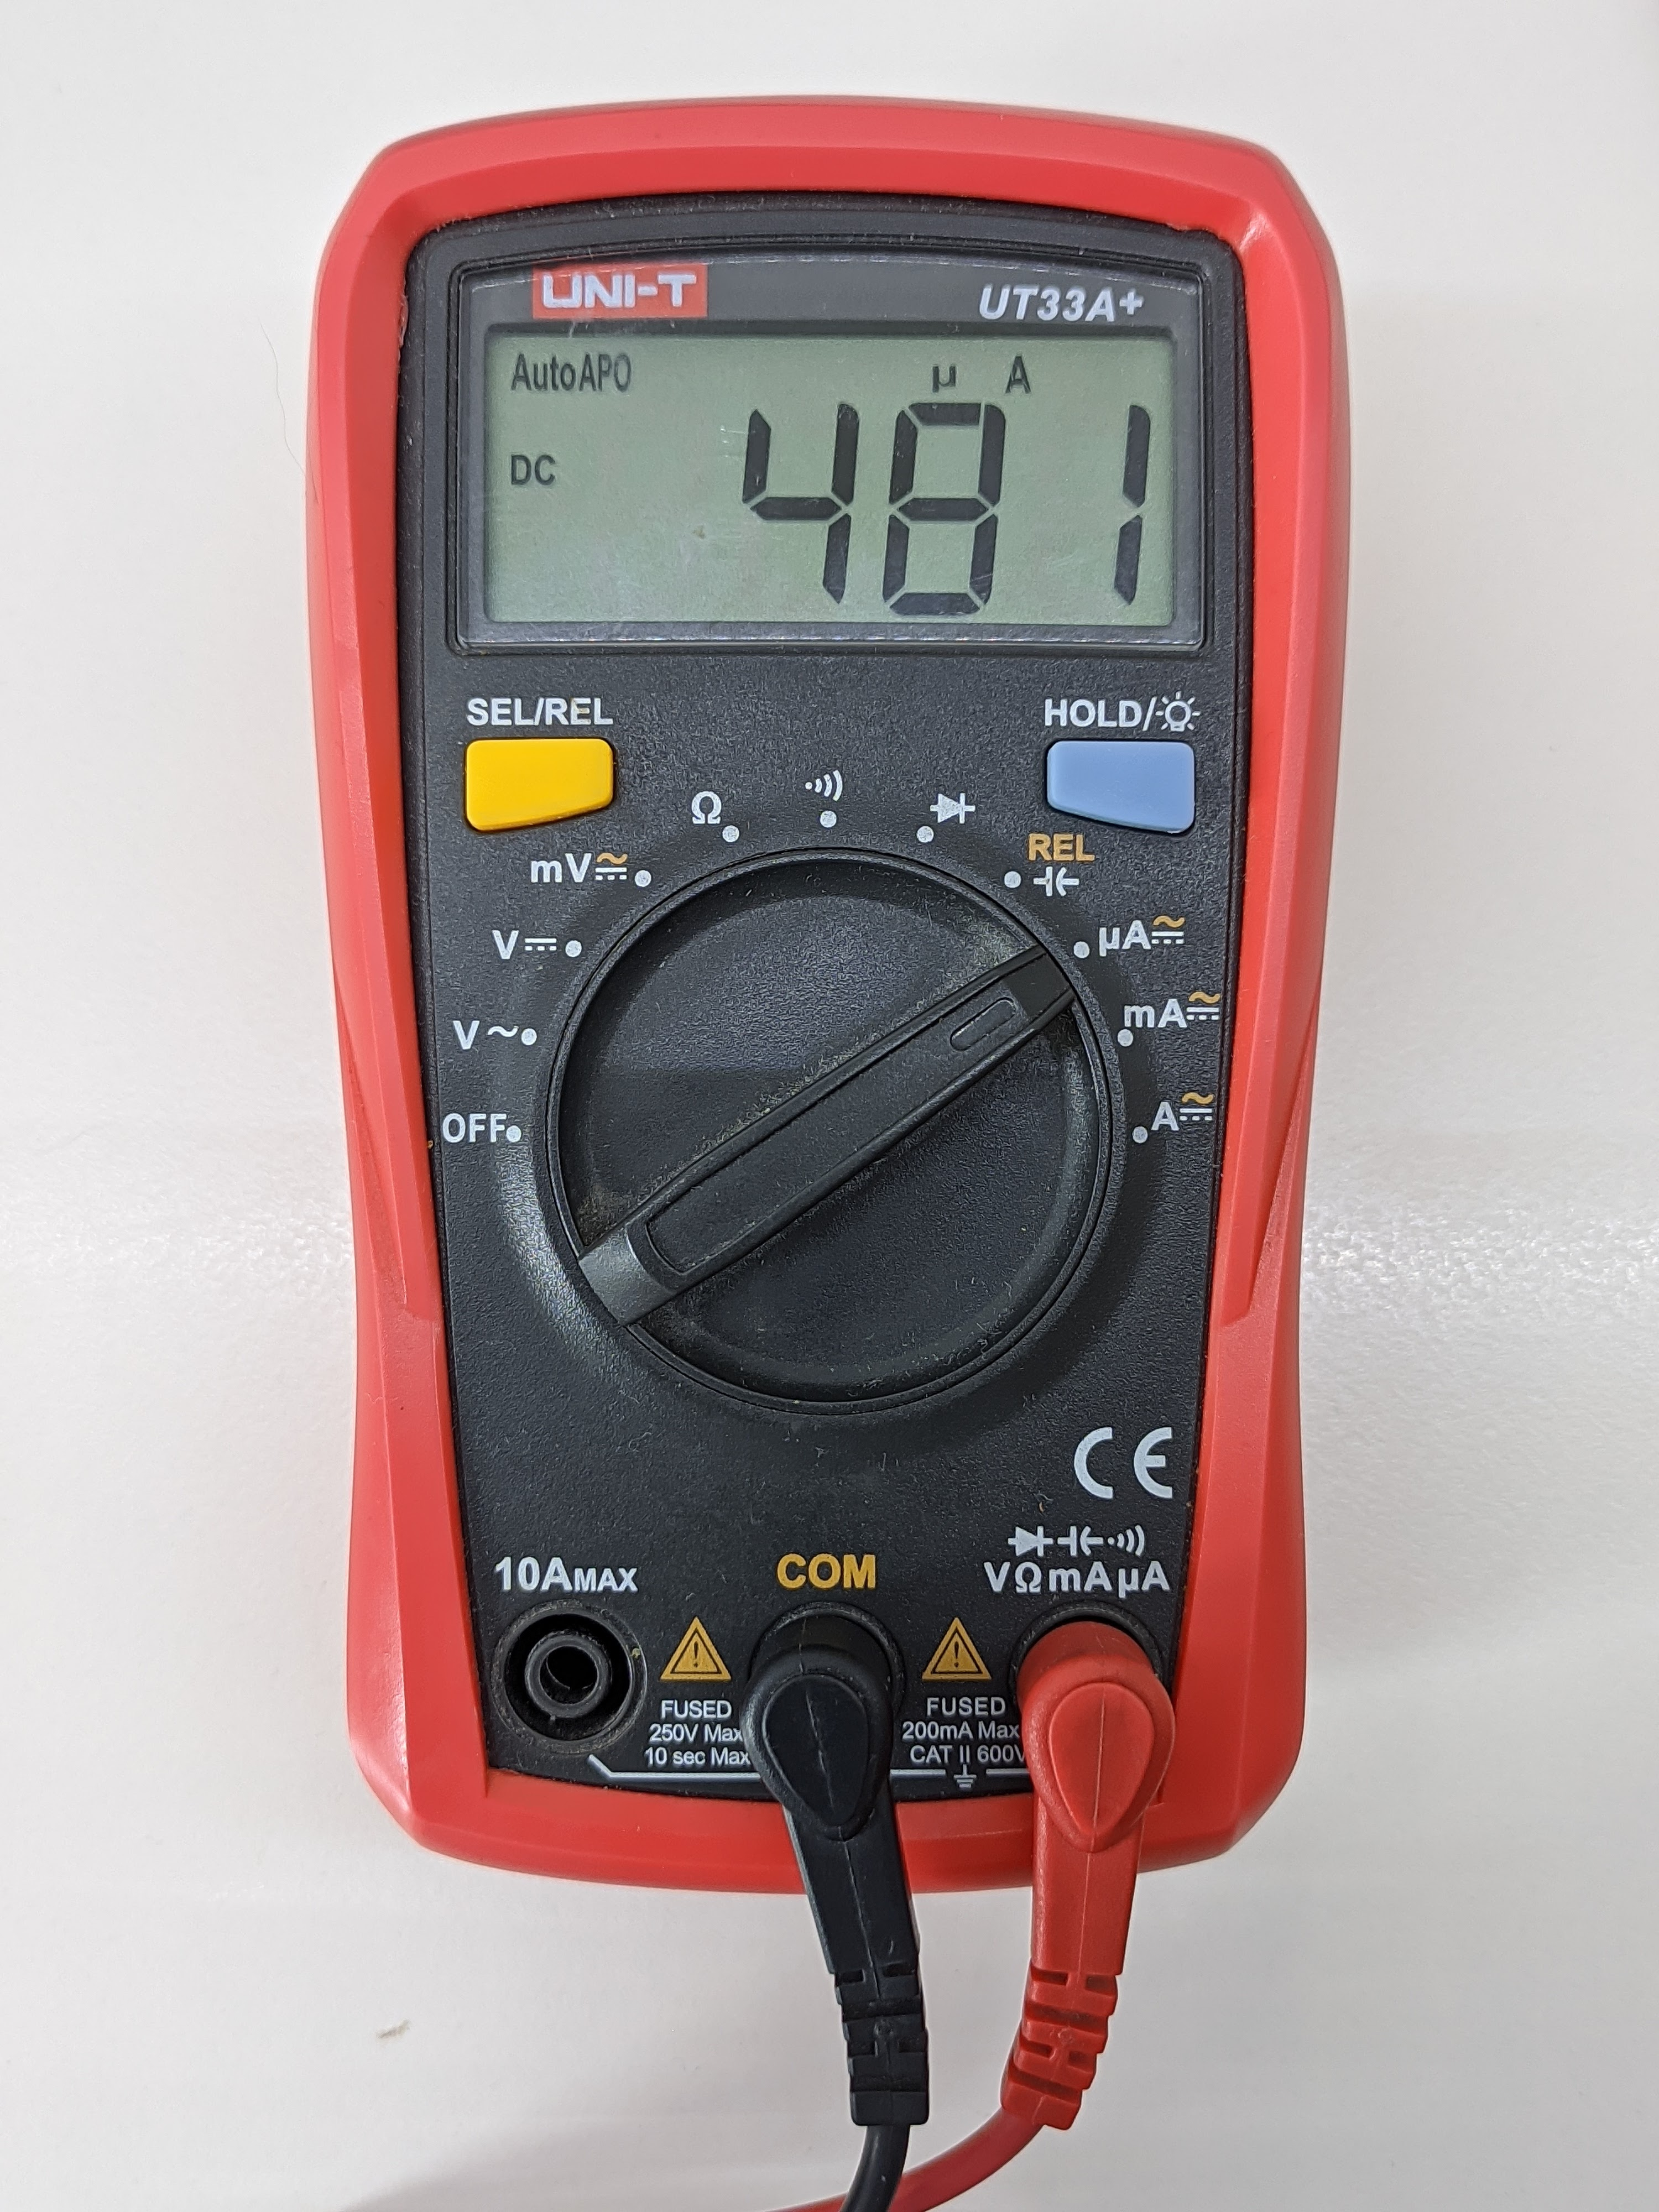
\includegraphics[width=1\linewidth]{pictures/mult-i3.jpg}
            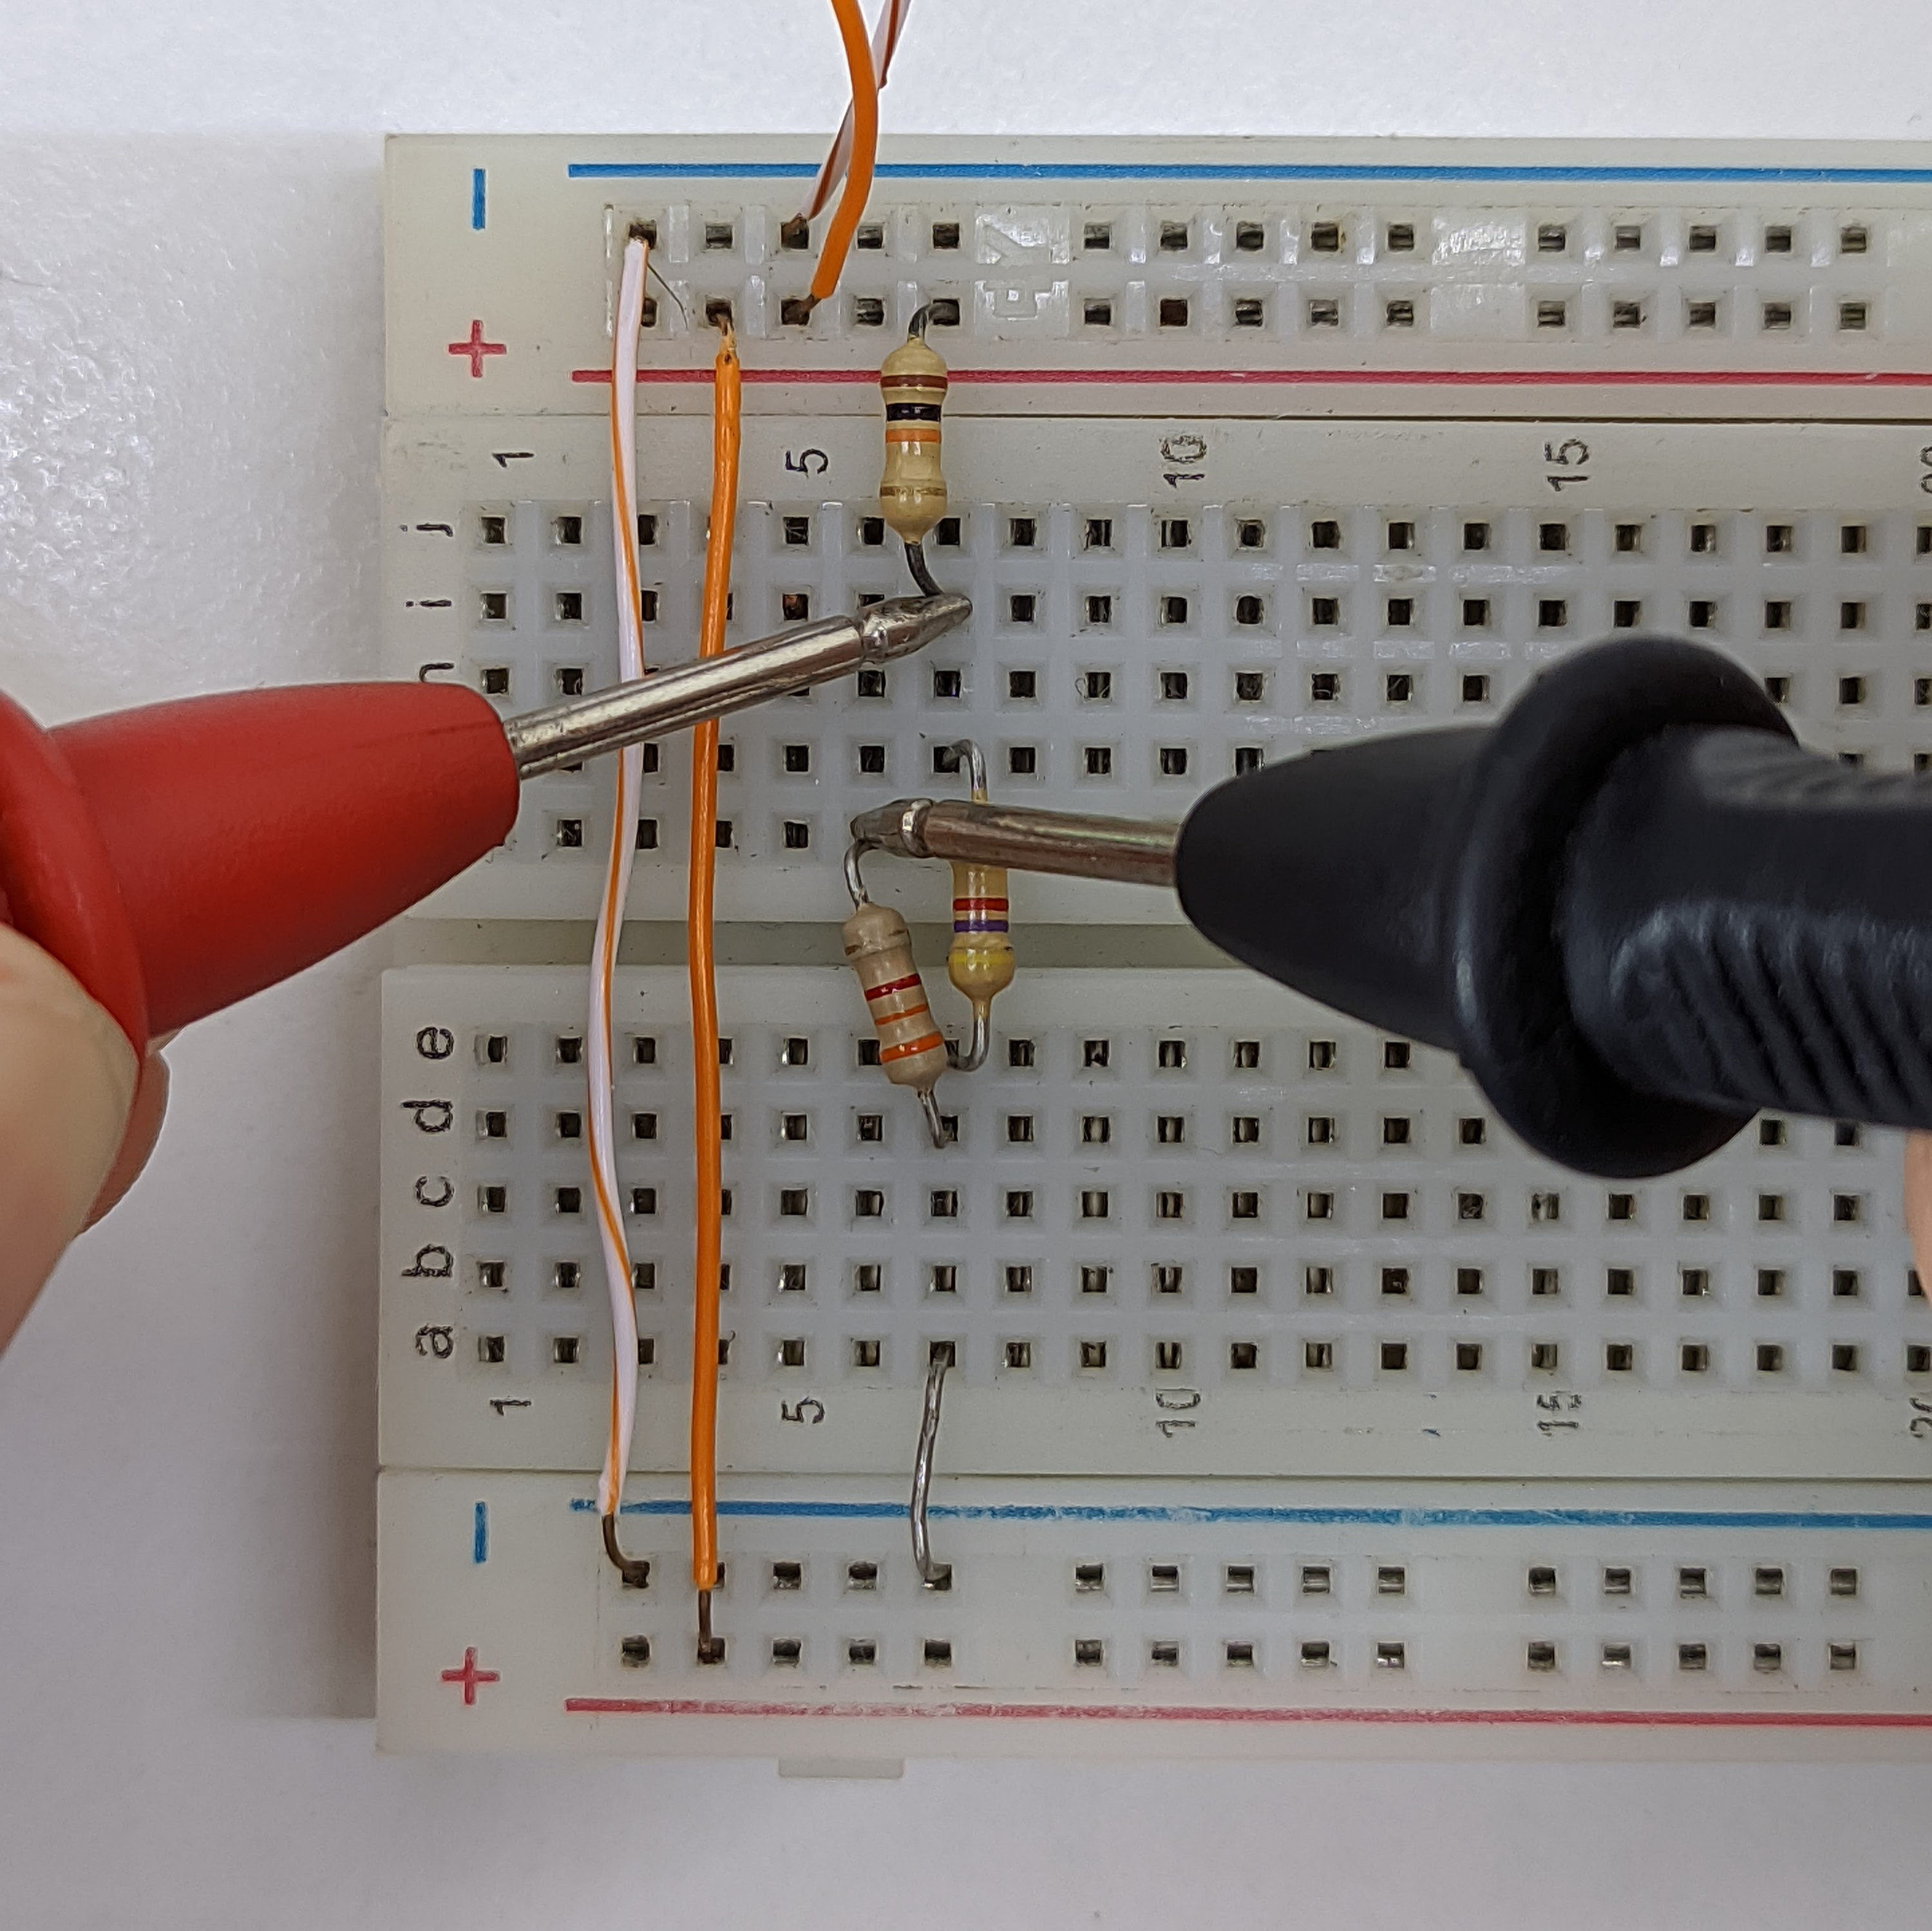
\includegraphics[width=1\linewidth]{pictures/prot-i3.jpg}
            \caption{Medición $I_3$.}
          \end{minipage}
      \end{figure}


      Con el objetivo de comparar, se presenta a continuación una tabla de los valores calculados con resistores y
      fuentes ideales y los valores medidos en la practica de laboratorio:
      \begin{figure}[!h]
        \centering
        \begin{tabular}[c]{|c||c|c|c|c||c|}
          \hline
          \multicolumn{6}{|c|}{Comparativa de valores}\\
          \hline
                    & $V_s$         & $R_1$         & $R_2$         & $R_3$         & \\
          \hline
          Tensión   & $10V$         & $8,3760V$     & \multicolumn{2}{|c||}{$1,6239V$} & \multirow{2}{*}{Ideal}\\
          \cline{1-5}
          Corriente &               & $837,6\mu A$  & $345,5\mu A$  & $492\mu A$    & \\
          \hline
          Tensión   & $9,98V$       & $8,36V$       & \multicolumn{2}{|c||}{$1,611V$}  & \multirow{2}{*}{Real}\\
          \cline{1-5}
          Corriente &               & $829\mu A$    & $340\mu A$    & $481\mu A$    & \\
          \hline
        \end{tabular}
      \end{figure}

      La precisión de los valores de la realidad con respecto a los ideales tiene que ver con las resistencias de
      contacto al colocar los elementos en la Protoboard y las puntas del multímetro, y las tolerancias de fabricación
      de los resistores (en este caso, 5\%).

    \myemptypage
    \chapter{Actividad Anexa}
      El profesor propuso, a modo de interiorizarse con las herramientas de trabajo del laboratorio, reemplazar la
      fuente de corriente continua por un generador de funciones. Este mismo, configurado a $10Vpp$, onda sinusoidal y
      frecuencia de $50Hz$ simula un transformador de corriente alterna. De esta forma, podemos emplear el Osciloscopio
      para poder ver como se comportan los resistores bajo corrientes alternas.

      \section{Simulación}
      Para la simulación utilizamos nuevamente el software LTSpice, esta vez con el comando spice .tran (transient
      analysis) con $0.04s$ de muestra para ver dos ciclos de la señal alterna:
      \begin{figure}[!h]
        \centering
        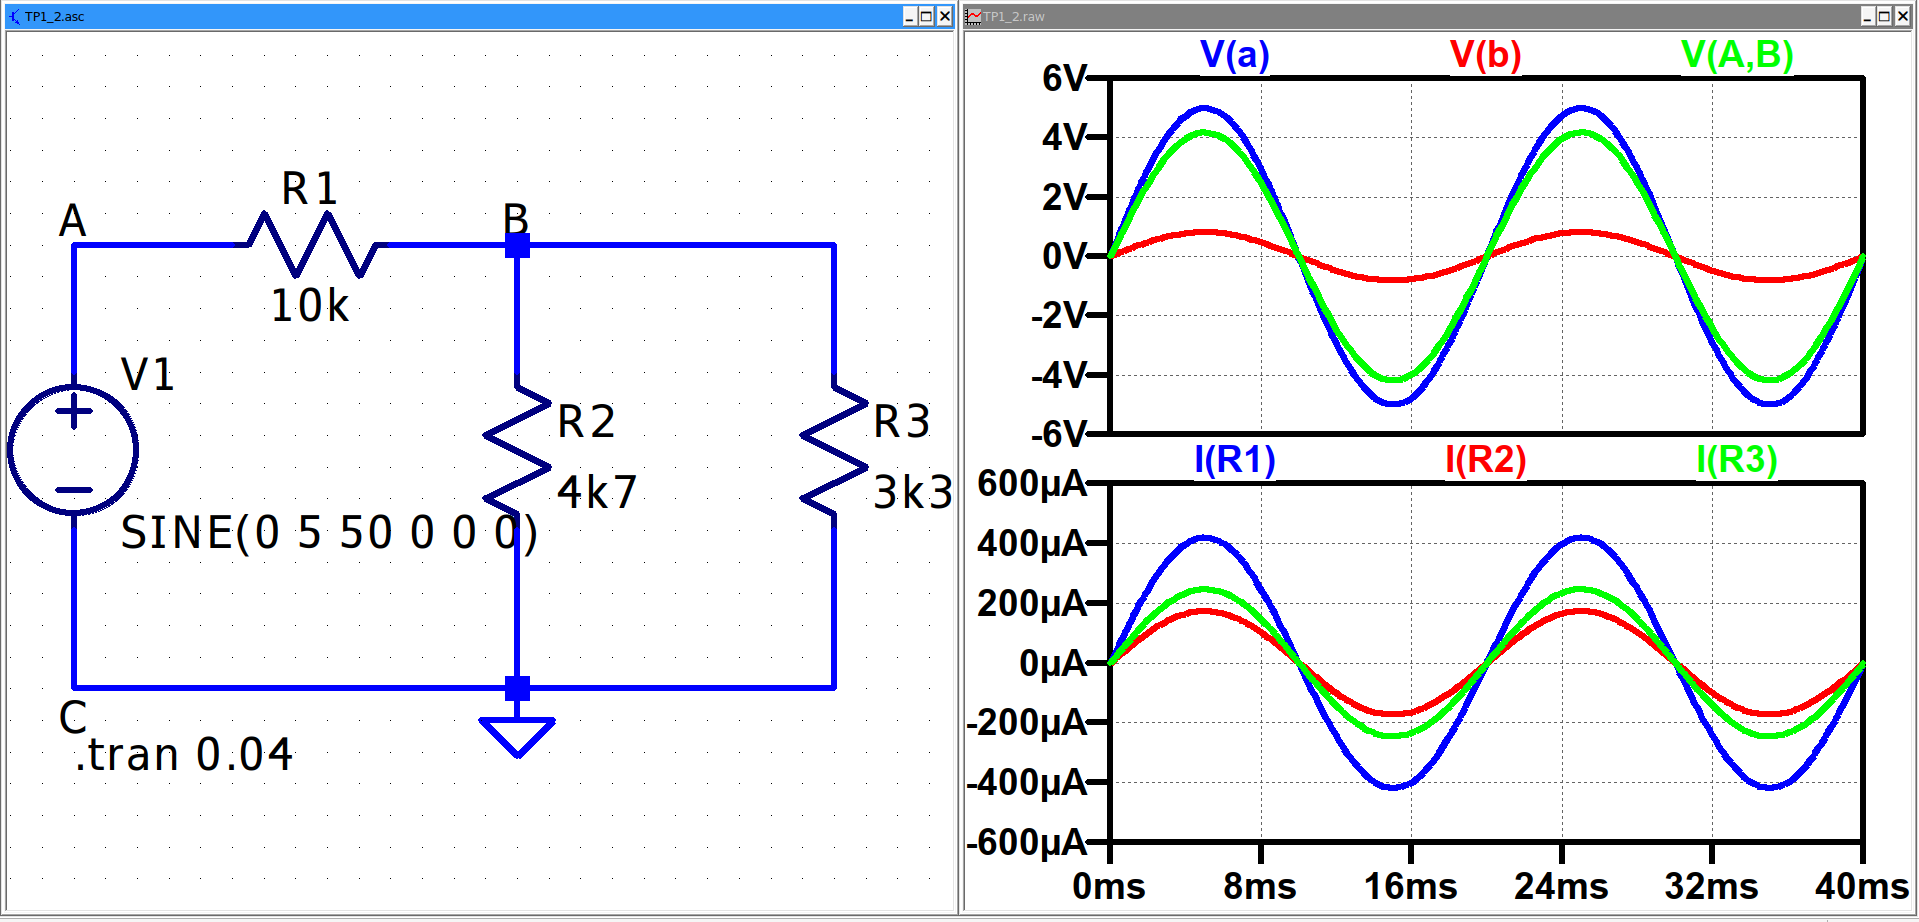
\includegraphics[width=1\linewidth]{images/sim_ac.png}
        \caption{Simulación en corriente alterna.}
      \end{figure}

      Podemos entonces observar que la caída de tensión pico-pico en el resistor $R_1$ es de aproximadamente $8,376V$,
      y en el resistor $R_2$ es de aproximadamente $1,623V$. Así mismo, las corrientes tienen valores pico-pico
      similares a los calculados en corriente continua. Para $i_t$ son $837,6\mu A$, para $i_2$, $345,4\mu A$ y para
      $i_3$, $491,9\mu A$.

      \newpage
      \section{Mediciones}
      Configurando el generador de funciones, y después de haber calibrado el osciloscopio, podemos ver la siguiente
      señal en el mismo:
      \begin{figure}[!h]
        \centering
        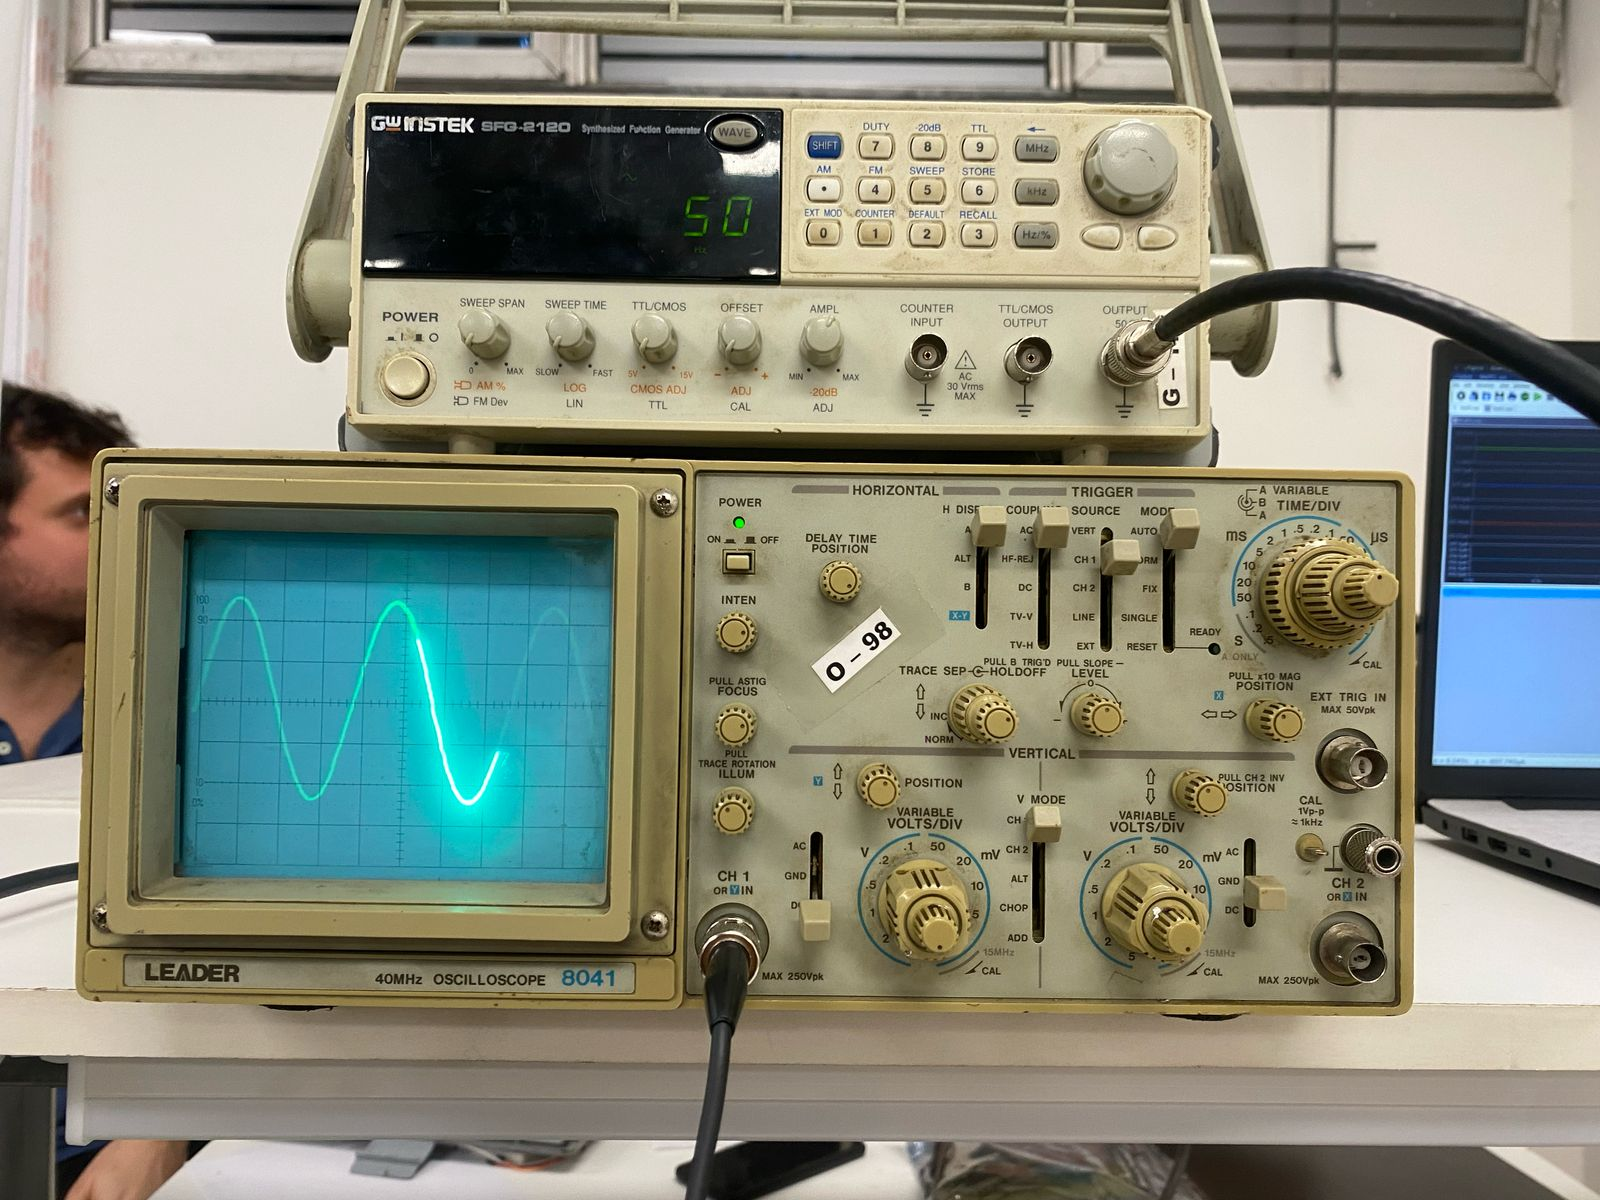
\includegraphics[width=0.8\linewidth]{pictures/osc-ac_vs.jpeg}
        \caption{Calibración del generador de funciones. Osciloscopio configurado a 2V/div, 5mS/div.}
      \end{figure}

      Si conectamos ahora la salida del generador de funciones a nuestro circuito, podemos observar las caídas de
      tensión en cada resistor:
      \begin{figure}[!h]
        \centering
        \begin{minipage}{0.45\textwidth}
          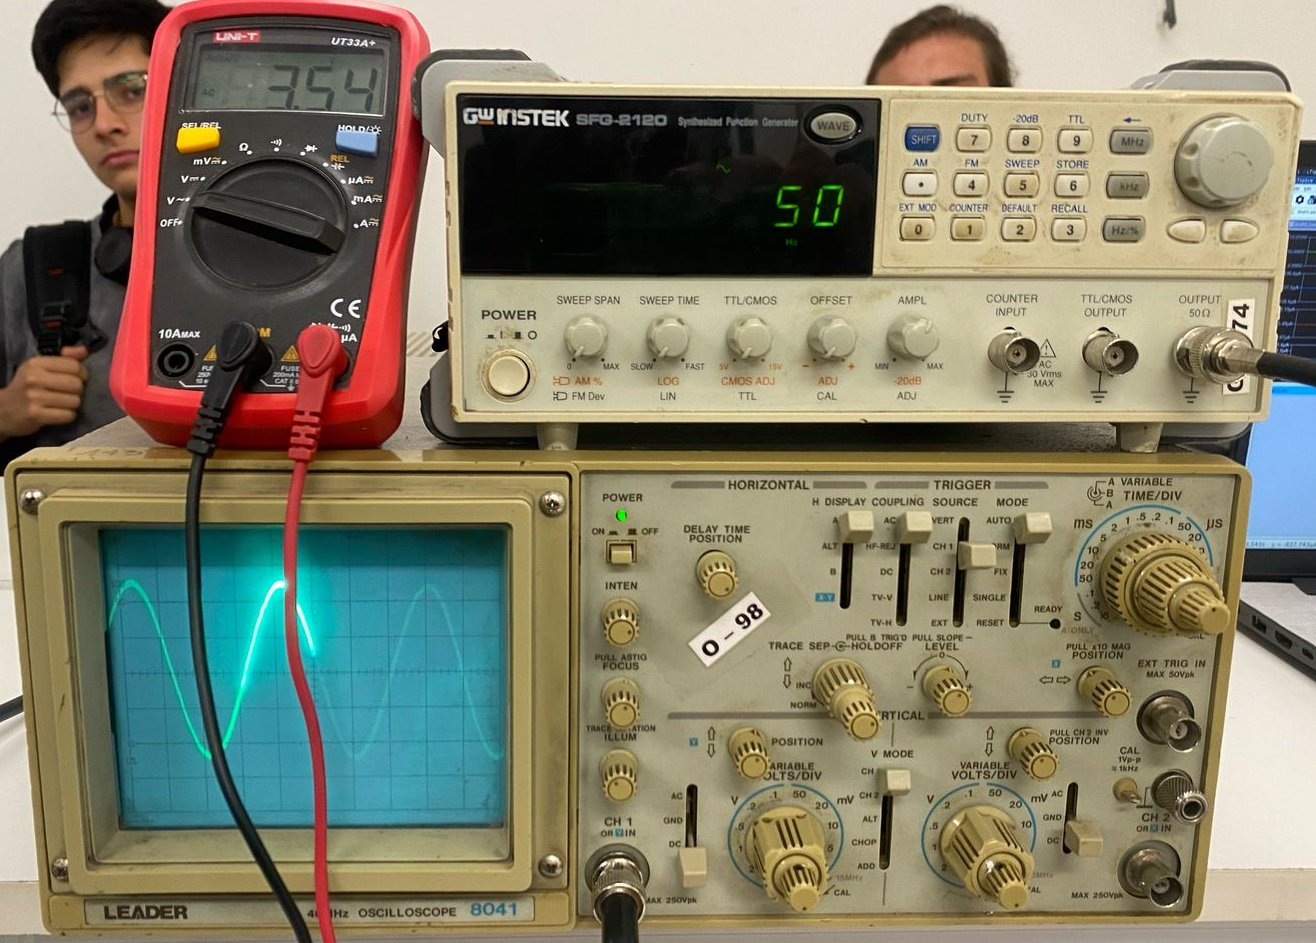
\includegraphics[width=1\linewidth]{pictures/osc-mult-ac_v_r1.jpeg}
          \caption{$V_{R_1}$. Osciloscopio configurado a 1V/div, 5mS/div. Lectura: $3,54V$}
        \end{minipage}
        \hspace{0.5cm}
        \begin{minipage}{0.45\textwidth}
          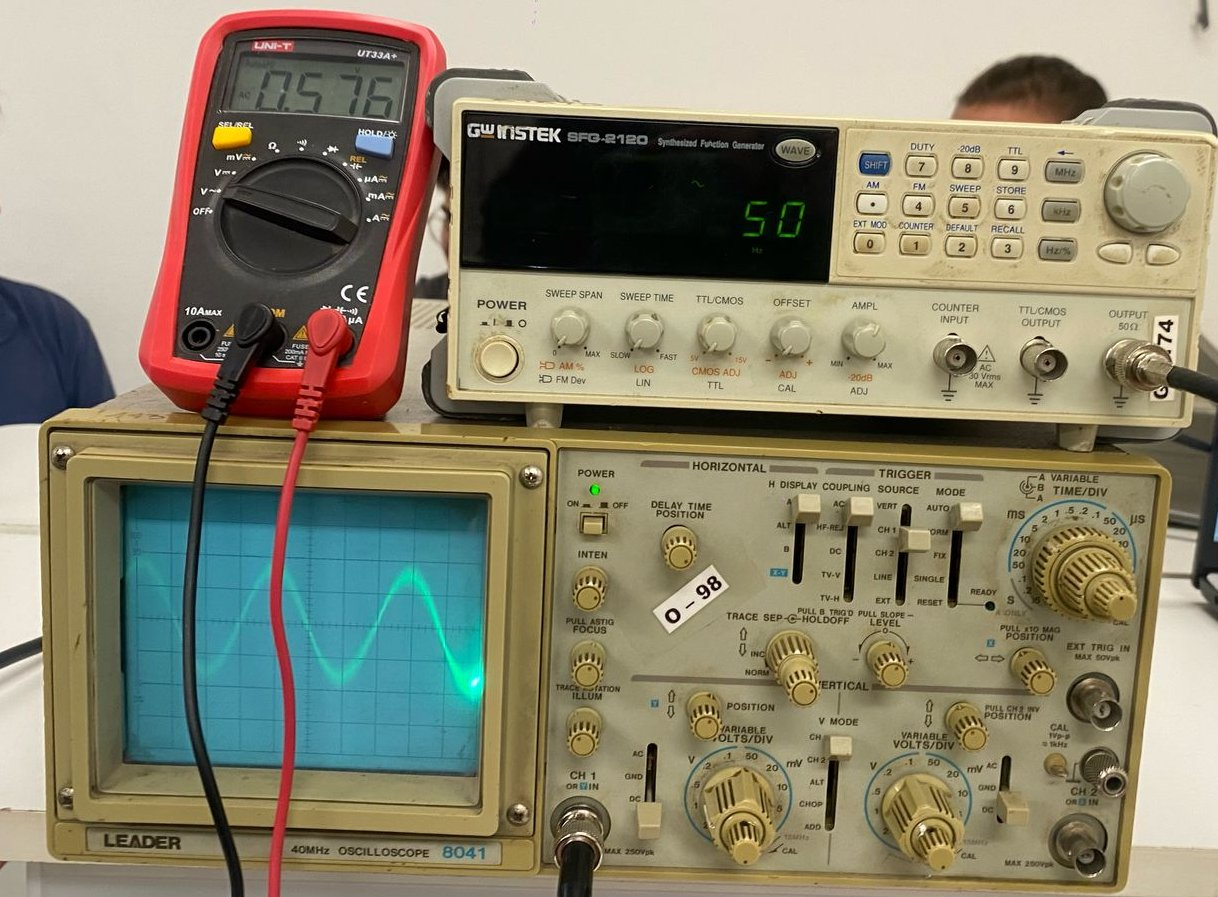
\includegraphics[width=1\linewidth]{pictures/osc-ac-mult-v_r2-r3.jpeg}
          \caption{$V_{R_2}$. Osciloscopio configurado a 1V/div, 5mS/div. Lectura: $0,576V$}
        \end{minipage}
      \end{figure}

      Naturalmente, los números no coinciden, esto es debido a que el multímetro esta midiendo el valor eficaz de la
      caída de tensión en las resistencias, y no el valor pico o el valor pico-pico. Así y todo, al momento de escribir
      el informe, quisimos corroborar esas mediciones, y nos dimos cuenta que posiblemente hayamos calibrado mal el
      osciloscopio, y por lo tanto el generador de funciones, ya que los valores eficaces, pasados a valores pico-pico,
      no se acercan por algunos volts a los valores simulados.

    \chapter{Conclusión}
      Este trabajo práctico nos permitió aplicar los conceptos teóricos de circuitos resistivos y familiarizarnos con
      herramientas clave como el multímetro, el osciloscopio y el generador de funciones. Durante las mediciones,
      aprendimos a configurar correctamente el osciloscopio para visualizar señales, aunque enfrentamos posibles
      errores como la mala calibración de las escalas, lo que posiblemente afecto la precisión de las lecturas.

      Los desafíos principales incluyeron la calibración precisa de la fuente y las variaciones en las mediciones
      debido a tolerancias de componentes y resistencias de contacto. Los cálculos teóricos, respaldados por la
      simulación en LTSpice, mostraron una buena correlación con los valores prácticos, aunque con pequeñas
      discrepancias atribuibles a las no idealidades de los elementos reales.

      Las mediciones confirmaron que, a pesar de las diferencias (como el 2-3\% en las corrientes), los resultados
      fueron consistentes con lo esperado, validando tanto la metodología empleada como los principios fundamentales
      de la ley de Ohm y las ecuaciones de malla. Esta experiencia reforzó la importancia de considerar factores
      prácticos en el diseño y análisis de circuitos, así como la utilidad de las herramientas de simulación para
      anticipar resultados.

      En definitiva, el trabajo cumplió con su objetivo principal: integrar teoría, simulación y práctica, destacando
      la relevancia de la precisión en las mediciones y el manejo de incertidumbres en electrónica básica. La actividad
      anexa nos permitió desarrollar habilidades en el uso de instrumentos de laboratorio, aunque también nos alertó
      sobre posibles fuentes de error, como la configuración del osciloscopio o las conexiones mal realizadas.

      \myemptypage
    \chapter{Anexos}
      \section{Rubrica}
      \begin{figure}[!h]
        \centering
        \begin{tabular}[c]{|c|c|c|}
          \rowcolor{gray!30}
          \hline
          \textbf{Tarea}                      & \textbf{Puntuación} & \textbf{Máximo}\\
          \hline
          Presentación del informe            &                     & 30\%\\
          \hline
          Explicación del proceso de medición &                     & 40\%\\
          \hline
          Defensa de las conclusiones         &                     & 30\%\\
          \hline
          \textbf{Total}                      &                     & \textbf{100\%}\\
          \hline
        \end{tabular}
      \end{figure}

      \section{Planilla de Seguimiento}
      \begin{figure}[!h]
        \begin{footnotesize}
          \begin{tabular}{|m{1cm}|m{1cm}|m{1.3cm}|m{2cm}|m{1.7cm}|m{1.7cm}|m{1.7cm}|m{1.7cm}|m{1.7cm}|}
            \hline
            Versión del TP & Fecha de Inicio & Revisado Por & Resumen Observaciones Correcciones &
            Fecha de retroalimentación enviada & Cambios realizados por JTP? & Nueva fecha de entrega &
            Aprobado por jefe de cátedra?\\
            \hline
            1.0 (2025) & & & & & & &\\
            \hline
          \end{tabular}
        \end{footnotesize}
      \end{figure}

\end{document}
